\documentclass[entropy,article,submit,moreauthors,pdftex]{Definitions/mdpi}
    %[english,sort&compress]{elsarticle}



% ------------------------- MDPI internal commands -------------------------- %
% --------------------------------------------------------------------------- %

\firstpage{1} 
\makeatletter 
\setcounter{page}{\@firstpage} 
\makeatother
\pubvolume{1}
\issuenum{1}
\articlenumber{0}
\pubyear{2021}
\copyrightyear{2020}
%\externaleditor{Academic Editor: Firstname Lastname} % For journal Automation, please change Academic Editor to "Communicated by"
\datereceived{} 
\dateaccepted{} 
\datepublished{} 
\hreflink{https://doi.org/} % If needed use \linebreak



% -------------------------- Packages inclusions ---------------------------- %
% --------------------------------------------------------------------------- %

\usepackage{bbm}
%\usepackage{amssymb,esint,tabularx}

\newcounter{GaussExample}% counter for the Gaussian example
\newcounter{qGaussExample}% counter for the qGaussian example
\newcounter{arcsineExample}% counter for the arcsine example
%\setcounter{}{}


%%%%%%%%%%%%%%%%%%%%%%%%%% TO SUPRESS FOR THE SUBMISSION %%%%%%%%%%%%%%%%%%%%%%
%%%%%%%%%%%%%%%%%%%%%%%%%%%%%%%%%%%%%%%%%%%%%%%%%%%%%%%%%%%%%%%%%%%%%%%%%%%%%%%
%%                                                                           %%
\usepackage{color}                                                           %%
\newcommand{\SZ}[1]{{\color{blue} #1}}                                       %%
\newcommand{\jfb}[1]{{\color{red} #1}}                                       %%
\newcommand{\Avoir}[1]{{\color{red}\bf #1}}                                  %%
%%                                                                           %%
%%%%%%%%%%%%%%%%%%%%%%%%%%%%%%%%%%%%%%%%%%%%%%%%%%%%%%%%%%%%%%%%%%%%%%%%%%%%%%%
%%%%%%%%%%%%%%%%%%%%%%%%%%%%%%%%%%%%%%%%%%%%%%%%%%%%%%%%%%%%%%%%%%%%%%%%%%%%%%%



% ---------------------- User specified LaTeX commands ----------------------- %
% ---------------------------------------------------------------------------- %

\def\dmu{\mathrm{d}\mu}% dmu with measure mu
\def\fB{\mathcal{B}}% functional Bregmann
\def\Rset{\mathbb{R}}% Real numbers
\def\X{\mathcal{X}}% set for r.v. X
\def\Y{\mathcal{Y}}% phi(X)
\def\D{\mathcal{D}}% set of distributions
\def\un{\mathbbm{1}}% indicator
\def\W{\operatorname{W}} % Lambert-W function
\def\argtanh{\operatorname{argtanh}}% arg tanh (or tanh^{-1})
\def\div{\operatorname{div}}% operator divergence
\DeclareMathOperator*{\argmax}{\operatorname{argmax}}% operator argmax
\newcommand{\Esp}[1]{\mathbb{E}\left[ #1 \right]}% math. mean
\newcommand{\hypgeom}[2]{\mbox{}_{#1}\hspace{-1pt}F_{#2}}% hypergeom function
\def\u{\mathrm{u}}
%\def\m{\mathrm{m}}


% -------------------------------- Frontpage --------------------------------- %
% ---------------------------------------------------------------------------- %

\Title{$\phi$-informational  measures:  some results and interrelations}
\TitleCitation{$\phi$-informational  measures:  some results  and interrelations}
%
\newcommand{\orcidauthorA}{0000-0001-7595-9601}
%\newcommand{\orcidauthorB}{0000-0001-7595-9601}
\Author{Steeve Zozor $^{1,*}$\orcidA{} and Jean-Fran\c{c}ois Bercher $^{2}$}
\AuthorNames{Steeve Zozor and Jean-Fran\c{c}ois Bercher}
\AuthorCitation{Zozor, S.; Bercher, J.-F.}
%
\address{%
  $^1$ \quad  Univ. Grenoble  Alpes, CNRS,  Grenoble INP*,  GIPSA-Lab,
  38000  Grenoble,  France\newline  *Institute  of  Engineering  Univ.  Grenoble
  Alpes\newline steeve.zozor@cnrs.fr\\
%
  $^2$  \quad   LIGM,  Univ  Gustave  Eiffel,   CNRS,  F-77454  Marne-la-Vallée,
  France\newline jean-francois.bercher@esiee.fr
  %
}

\corres{Correspondence: steeve.zozor@cnrs.fr}
%Tel.:  (optional; include  country code;  if there  are multiple  corresponding
%authors, add author initials) +xx-xxxx-xxx-xxxx (F.L.)}

% Current address and/or shared authorship
%\firstnote{Current address: Affiliation 3} 
%\secondnote{These authors contributed equally to this work.}



% --------------------------------- Abstract --------------------------------- %
% ---------------------------------------------------------------------------- %

\abstract{In this paper  we focus on extended informational measures  based on a
  convex function  $\phi$~: entropies, extended Fisher  information, generalized
  moments.  Both  the generalization of  the Fisher information and  the moments
  are based on the definition of  an escort distribution, precisely based on the
  (entropic)  functional $\phi$.   We  thus revisit  the  usual maximum  entropy
  principle   --more  especially   its  inverse   problem,  starting   from  the
  distribution  and constraints--,  which conduct  to a  wider extension  of the
  $\phi$-entropy  with   a  state-dependent   entropic  functional.    Then,  we
  generalize  some interrelations  between the  extended informational  measures
  such that Cram\'er-Rao inequalitie and the  de Bruijn identity in this broader
  context.  In this particular framework, the maximum entropy distributions play
  en central role.  All the results derived  in the paper include the usual ones
  as special cases.}



% --------------------------------- Keywords --------------------------------- %
% ---------------------------------------------------------------------------- %

\keyword{$\phi$-entropy;   state-dependent  $\phi$-entropy;   (inverse)  maximum
  $\phi$-entropy    problem;    $\phi$-escort    distributions;    $\phi$-Fisher
  information; $\phi$-moments; generalized  Cram\'er-Rao inequality; $\phi$-heat
  equation; generalized de Bruijn identity.}



% ---------------------------------------------------------------------------- %
% ------------------------- Beginning of the document ------------------------ %
% ---------------------------------------------------------------------------- %

\sloppy

\begin{document}



% ---------------------------------- MaxEnt ---------------------------------- %

\section{Introduction}
\label{sec:Intro}

Since  the  pioneer  works of  von  Neuman~\cite{vNeu27},  Shannon~\cite{Sha48},
Boltzmann, Maxwell, Planck and Gibbs~\cite{Bol64, Bol96, Bol98, Pla15, Nie52:v2,
  Jay65,  MulMul09} on  the entropy  as a  tool for  uncertainty or  information
measure, many investigations were devoted to the generalization of the so-called
Shannon entropy and its associated measures~\cite{Ren61, Var66, HavCha67, Csi67,
  Dar70, AczDar75,  DarJar79, Tsa88,  Sal87, SalMen93, Sal94,  LieVaj06, Bas13}.
If the Shannon measures are  compelling, especially in the communication domain,
for compression purposes, many generalizations proposed later on has also showed
promising   interpretations    and   applications   (Panter-Dite    formula   in
quantification    where     the    R\'enyi    or     Havdra-Charv\'at    entropy
emerges~\cite{PanDit51, Llo82, GerGra92}, codification penalizing long codewords
where the R\'enyi entropy appears~\cite{Cam65,  Ber09} for instance).  The great
majority of  the extended entropies  found in the  literature belongs to  a very
general  class  of  entropic measures  called  $(h,\phi)$-entropies~\cite{Csi67,
  BurRao82, SalMen93,  Sal94, MenMor97, Par06}.   Such a general class  (or more
precisely the subclass of $\phi$-entropies) traced back to the work of Burbea \&
Rao~\cite{BurRao82}. They  offer not only  a general framework to  study general
properties  shared by  special entropies,  but  they also  offer many  potential
applications as  described for instance  in~\cite{Par06}.  Note that if  a large
amount of work deals with divergences, entropies occur as special cases when one
takes a uniform reference measure.

In the  settings of these  generalized entropies, the so-called  maximum entropy
principle takes  a special place.   This principle, advocated by  Jaynes, states
that  the  statistical  distribution  that describes  a  system  in  equilibrium
maximizes the entropy while satisfying  the system's physical constraints (e.g.,
the  center of  mass, energy)~\cite{Jay57,  Kap89, Arn01,  CovTho06, Gok75}.  In
other  words, it  is  the less  informative  law given  the  constraints of  the
system. In the Bayesian approach, dealing  with the stochastic modeling of a
parameter, such a principle (or a minimum divergence principle) is often used to
choose  a  prior  distribution  for  the  parameter~\cite{Jay68,  Csi91,  Bas13,
  FriSri08, Rob07}. It also finds  its counterpart in communication, clustering,
pattern recognition,  problems, among many others~\cite{Kap89,  Jay82, JonByr90,
  Arn01,  HerMa02, ParBer09}.   In  statistics, some  goodness-of-fit tests  are
based on  entropic criteria derived  from the  same idea of  constrained maximal
entropic  law~\cite{Vas76, Gok83,  Son02, Leq14,  Leq15, GirReg15}.  In a  large
number of  works using the  maximum entropy principle,  the entropy used  is the
Shannon entropy, although several extensions  exist in the literature.  However,
if for some reason a generalized entropy is considered, the approach used in the
Shannon   case  does   not  fundamentally   change~\cite{KesKap89,  BorLew91:03,
  BorLew91:05, BorLew93}.

One  can consider  the  inverse problem  which consists  in  finding the  moment
constraints  leading  to   the  observed  distribution  as   a  maximal  entropy
distribution~\cite{KesKap89}.  Kesavan \& Kapur  also envisaged a second inverse
problem, where both the distribution and the moments are given.  The question is
thus to determine  the entropy so that  the distribution is its  maximizer. As a
matter  of fact,  dealing with  the  Shannon entropy,  whatever the  constraints
considered,  the   maximum  entropy   distribution  falls  in   the  exponential
family~\cite{CovTho06, BorLew91:05, Arn01,  MezMon09}.  Considering more general
entropies  allows to  escape from  this  limitation.  Moreover,  if the  Shannon
entropy  (or the  Gibbs entropy  in physics)  is well  adapted to  the study  of
systems in the  equilibrium (or in the thermodynamic  limit), extended entropies
allow a finer  description of systems out  of equilibrium~\cite{Tsa88, TsaMen98,
  Tsa99,  Tsa09, EssSch00,  ParBir05}, exhibiting  their importance.   While the
problem  was considered  mainly  in the  discrete setting  by  Kesavan \&  Kapur
in~\cite{KesKap89},  \SZ{we will  recall  it  in the  general  framework of  the
  $\phi$-entropies probability densities with respect to any reference measure,}
and make a further step considering an extended class of these entropies.


While  the  entropy is  a  widely  used  tool  for quantifying  information  (or
uncertainty) attached  to a  random variable or  to a  probability distribution,
other quantities are used  as well, such as the moments  of the variable (giving
information  for instance  on center  of mass,  dispersion, skewness,  impulsive
character), or  the Fisher information.   In particular, the  Fisher information
appears in the context of  estimation~\cite{Kay93, Fri04}, in Bayesian inference
through the  Jeffreys prior~\cite{Rob07, Jef46},  but also for  complex physical
systems  descriptions~\cite{Fri04,   VigBer03,  RomAng99,   RomSan06,  SanGon06,
  TorLop15}.


Although  coming from  different worlds  (information theory  and communication,
estimation, statistics,  physics), these informational quantities  are linked by
well-known  relations  such  as  the  Cram\'er-Rao  inequality,  the  de  Bruijn
identity, the Stam inequality~\cite{CovTho06, Sta59, DemCov91, GuoSha05}.  These
relationships have  been proved very  useful in  various areas, for  instance in
communications~\cite{Sta59, DemCov91,  CovTho06}, in  estimation~\cite{Kay93} or
in physics~\cite{FolSit97, Sen11}, among others.  When generalized entropies are
considered,  it  is  natural  to  question  the  other  informational  measures'
generalization and the associated identities or inequalities. This question gave
birth  to   a  large  amount   of  work  and  is   still  an  active   field  of
research~\cite{Vaj73,  Boe77,  Ham78,  BoeVan80, BurRao82,  LutYan04,  LutYan05,
  LutYan07, LutLv12, Ber12:06_1, Ber12:06_2, Ber13, Ber13:08}.

In this  paper, we show that  it is possible  to build a whole  framework, which
associates  a  target maximum  entropy  distribution  to generalized  entropies,
generalized moments  and generalized  Fisher information.   In this  setting, we
derive generalized inequalities and  identities relating these quantities, which
are all linked in some sense to the maximum entropy distribution.


\

The paper is organized as  follows. In section~\ref{sec:MaxPhiEnt} we recall the
definition of the generalized $\phi$-entropy.  Thus, we come back to the maximum
entropy   problem   in   this    general   settings.    Following   the   sketch
of~\cite{KesKap89},  we  present a  sufficient  condition  linking the  entropic
functional and  the maximizing distribution,  allowing to both solve  the direct
and the inverse  problems.  When the sufficient conditions  linking the entropic
function and the distribution cannot be  satisfied, the problem can be solved by
introducing  state-dependent  generalized entropies,  which  is  the purpose  of
section~\ref{sec:MultiformEnt}.   In  section~\ref{sec:EscortCR},  we  introduce
informational quantities associated to the generalized entropies of the previous
sections, such that  a generalized escort distribution,  generalized moments and
generalized  Fisher informations.   These  generalized informational  quantities
allow to  extend the  usual informational relations  such that  the Cram\'er-Rao
inequality, relations saturated (or valid) dealing precisely for the generalized
maximum entropy  distribution.  Finally, in section~\ref{sec:deBruijn},  we show
that the  extended quantities allows to  obtain an extended de  Bruijn identity,
provided the distribution  follows a non-linear heat equation.   Some example of
determination of  $\phi$-entropies solving  the inverse maximum  entropy problem
are provided  in a  short series of  appendix, showing in  other that  the usual
quantities are recovered in the well known cases (Gaussian distribution, Shannon
entropy, Fisher information, variance).

\

In what follows,  we will define a series of  generalized information quantities
relative to  a probability  density defined  with respect  to a  given reference
measure $\mu$  (e.g., the Lebesgue  measure when dealing with  continuous random
variables,  discrete   measure  for  discrete-state   random  variables,\ldots).
Therefore, rigorously, all  these quantities depend on the  particular choice of
this reference  measure. However, for simplicity,  we will omit to  mention this
dependence in the notation along the paper.



% ----------------------------- Max (h,phi)-Ent ------------------------------ %

\section{$\phi$-entropies -- direct and inverse maximum entropy problems}
\label{sec:MaxPhiEnt}

Let  us  first  recall  the   definition  of  the  generalized  $\phi$-entropies
introduced by Csisz\`ar in terms of divergence,  and by Burbea and Rao in terms
of entropy:


\begin{Definition}[$\phi$-entropy~\cite{BurRao82}]
\label{def:phi-entropy}
  %
  Let $\phi: \Y \subseteq \Rset_+ \mapsto \Rset$ be a convex function defined on
  a convex  set $\Y$.  Then, if  $f$ is a probability  distribution defined with
  respect to a general  measure $\mu$ on a set $\X  \subseteq \Rset^d$ such that
  $f(\X) \subseteq \Y$, when this quantity exists,
  %
  \begin{equation}\label{eq:phi-entropy}
    H_{\phi}[f] = - \int_\X \phi(f(x)) \, \dmu(x)
  \end{equation}
  %
  is  the $\phi$-entropy  of  $f$.
\end{Definition}
%
The $(h,\phi)$-entropy is defined by $H_{(h,\phi)}[f] = h\left(H_\phi[f]\right)$
where $h$ is  a nondecreasing function.  The definition is  extended by allowing
$\phi$  to be  concave, together  with $h$  nonincreasing~\cite{Csi67, SalMen93,
  Sal94, MenMor97,  Par06}.  If  additionally $h$ is  concave, then  the entropy
functional $H_{(h,\phi)}[f]$ is concave.

\

Since  we are  interested in  the  maximum entropy  problem and  because $h$  is
monotone, we can  restrict our study to the  $\phi$-entropies.  Additionally, we
will assume that $\phi$ is {\em strictly} convex and {\em differentiable}.

\

A related  quantity is  the Bregman divergence  associated with  convex function
$\phi$:

%
\begin{Definition}[Bregman divergence and functional Bregman divergence~\cite{Bre67, Bas13}]
\label{def:Bregman}
%
  With  the  same  assumptions  as in  def.~\ref{def:phi-entropy},  the  Bregman
  divergence associated with $\phi$ defined on a convex set $\Y$ is given by the
  function defined on $\Y \times \Y$,
  %
  \begin{equation}\label{eq:Bregman}
    \SZ{B}_\phi(y_1,y_2) = \phi(y_1) - \phi(y_2) - \phi'(y_2) \left(y_1-y_2\right).
  \end{equation}
  %
  Applied  to two  functions  $f_i: \X  \mapsto  \Y$, $i=1,  2$, the  functional
  Bregman divergence writes
  \begin{equation}
  \label{eq:FctBregman}
  \SZ{\fB}_\phi(f_1,f_2)  =  \int_\X   \!  \phi(f_1(x))  \,  \dmu(x)   -  \int_\X  \!
  \phi(f_2(x))  \, \dmu(x)  - \int_\X  \! \phi'(f_2(x))  \left( f_1(x)  - f_2(x)
  \right) \, \dmu(x).
  \end{equation}
  %
  A direct consequence of the strict convexity of $\phi$ is the nonnegativity of
  the   (functional)   Bregman   divergence:   $\SZ{B}_\phi(y_1,y_2)   \ge   0$   and
  $\SZ{\fB}_\phi(f_1,f_2) \ge 0$, with equality if and only if $y_1 = y_2$ and $f_1 =
  f_2$ almost everywhere respectively.
\end{Definition}

More  generally,  the Bregman  divergence  is  defined for  multivariate  convex
functions,     where    the     derivative    is     replaced    by     gradient
operator~\cite{Bre67}. Extensions  for convex function of  functions also exist,
where the derivative  is in the sense of  G\^ateau~\cite{NieNoc17}. Such general
extensions are not  useful for our purposes; thus, we  restrict ourselves to the
above definition where $\Y \subseteq \Rset_+$.



% ---------------------------------------------------------------- MaxEnt direct

\subsection{Maximum entropy principle: the direct problem}
\label{subsec:MaxPhiEntDirect}

Let us first  recall the maximum entropy problem that  consists in searching for
the distribution maximizing the $\phi$-entropy~\eqref{eq:phi-entropy} subject to
constraints on  some moments $\Esp{T_i(X)}$  with $T_i: \Rset^d  \mapsto \Rset$,
$i=1,\ldots,n$. This direct problem writes
%
\begin{equation}\label{eq:MaxEnt}
\displaystyle f^\star \: = \argmax_{f \in \SZ{\D_{T,t}}} \left( - \int_\X \phi(f(x)) \,
\dmu(x) \right)
\end{equation}
%
with
%
\begin{equation}\label{eq:Ct}
\SZ{\D_{T,t}} = \left\{ f \ge 0: \: \Esp{T_i(X)} = t_i, i=0,\ldots,n\right\},
\end{equation}
%
where $T_0(x)  = 1$ and  $t_0 = 1$ (normalization  constraint)\SZ{, $T =  (T_0 ,
  \ldots , T_n), \, t = (t_0 , \ldots , t_n)$}.  The maximization problem being
strictly concave,  the solution exists and  is unique. A technique  to solve the
problem  can be  to use  the  classical Lagrange  multipliers technique  \SZ{and
  solving the  Euler-Lagrange equation from  the variational problem},  but this
approach   requires  mild   conditions~\cite{KesKap89,  BorLew91:03,   BorLew93,
  BenBor92,  TebVaj93,  Gir97}.   In  the following  proposition,  we  recall  a
sufficient  condition relating  $f$  and $\phi$  so that  $f$  is the  problem's
solution. Below, we prove the result without the use of the Lagrange technique.


\begin{Proposition}[Maximal $\phi$-entropy solution~\cite{KesKap89}]
\label{prop:sol-phi}
%
  Suppose that there exists a probability distribution $f \in \SZ{\D_{T,t}}$ satisfying
  %
  \begin{equation}\label{eq:sol-phi}
  \phi'\big(f(x)\big) = \sum_{i=0}^n \lambda_i \, T_i(x),
  \end{equation}
  %
  for  some $(\lambda_0,\ldots,\lambda_n)  \in \Rset^{n+1}$.   Then, $f$  is the
  unique solution of the maximal entropy problem~\eqref{eq:MaxEnt}.
\end{Proposition}
%
\begin{proof}
  Suppose that  distribution $f$  satisfies eq.~\eqref{eq:sol-phi}  and consider
  any distribution $g  \in \SZ{\D_{T,t}}$.  The functional Bregman  divergence between $f$
  and $g$ writes
  %
  \begin{eqnarray*}
  \SZ{\fB}_\phi(g,f) & = & \int_\X \phi(g(x)) \, \dmu(x) - \int_\X \phi(f(x)) \,
  \dmu(x) - \int_\X \phi'(f(x)) \left( g(x) - f(x) \right) \, \dmu(x)
  \\[2mm]
  & = & - H_\phi[g] + H_\phi[f] - \sum_{i=0}^n \lambda_i \int_\X T_i(x) \left(
  g(x) - f(x) \right) \, \dmu(x)
  \\[2mm]
  & = & H_\phi[f] - H_\phi[g]
  \end{eqnarray*}
  %
  where we  used the fact  that $g$ and  $f$ are both  probability distributions
  with the same  moments $\Esp{T_i(X)} = t_i$.  By nonnegativity  of the Bregman
  functional divergence, we finally get that
  %
  \[
  H_\phi[f] \ge H_\phi[g]
  \]
  %
  for all distribution  $g$ with the same  moments as $f$, with  equality if and
  only if  $g = f$ almost  everywhere.  In other  words, this shows that  if $f$
  satisfies eq.~\eqref{eq:sol-phi}, then it is the desired solution.
\end{proof}

Hence,  given  an entropic  functional  $\phi$  and moments  constraints  $T_i$,
eq.~\eqref{eq:sol-phi}  leads the  the maximum  entropy distribution  $f^\star$.
This distribution is parameterized by  the $\lambda_i$s or, equivalently, by the
moments $t_i$s.

Note  that  the reciprocal  is  not  necessarily  true,  as shown  for  instance
in~\cite{BorLew93}.   However,   the  reciprocal   is  true   when  $\X$   is  a
compact~\cite{Gir97} or for any $\X$ provided  that $\phi$ is locally bounded on
$\X$~\cite{Gir07}.




% --------------------------------------------------------------- MaxEnt inverse

\subsection{Maximum entropy principle: the inverse problems}
\label{subsec:MaxPhiEntInverse}

As stated in  the introduction, two inverse problems can  be considered starting
from a  given distribution  $f$. These  problems were  considered by  Kesavan \&
Kapur in~\cite{KesKap89} in the discrete framework.

\

The first inverse problem consists in searching for the adequate moments so that
a  desired distribution  $f$  is the  maximum entropy  distribution  of a  given
$\phi$-entropy.   This   amounts  to  find  functions   $T_i$  and  coefficients
$\lambda_i$ satisfying eq.~\eqref{eq:sol-phi}.  This is not always an easy task,
and even not  always possible. For instance,  it is well known  that the maximum
Shannon entropy  distribution given moment  constraints fall in  the exponential
family~\cite{CovTho06, BorLew91:05, Arn01, MezMon09}. Therefore, if $f$ does not
belong to this family, the problem has no solution.


\

The second  inverse problem consists  in designing  the entropy itself,  given a
target  distribution  $f$  and  given  the $T_i$s.   In  other  words,  given  a
distribution  $f$, eq.~\eqref{eq:sol-phi}  may allow  to determine  the entropic
functional $\phi$ so that $f$ is its maximizer.

As  for the  direct problem,  in  the second  inverse problem,  the solution  is
parameterized  by the  $\lambda_i$s. Here,  required properties  on $\phi$  will
shape the domain the $\lambda_i$s live in. In particular, $\phi$ must satisfy:
%
\begin{itemize}
\item the  domain of definition  of $\phi'$ must  include $f(\X)$; this  will be
  satisfied by construction;
%
\item from  the strict convexity  property of  $\phi$, $\phi'$ must  be strictly
  increasing.
\end{itemize}
%
Hence,  because $\phi'$  must  be  strictly increasing,  its  clear that  solving
eq.~\eqref{eq:sol-phi} requires the following two conditions:
%
\begin{enumerate}[label=(C\arabic*)]
\item\label{MonotonyDomains:cond}   $f(x)$   and   $\displaystyle   \sum_{i=1}^n
  \lambda_i  \, T_i(x)$  must  have the  same  variations, i.e.,  $\displaystyle
  \sum_{i=0}^n \lambda_i \, T_i(x)$  is increasing (resp.  decreasing, constant)
  where $f$ is increasing (resp. decreasing, constant);
%
\item\label{LevelSets:cond} $f(x)$ and  $\displaystyle \sum_{i=1}^n \lambda_i \,
  T_i(x)$ must have the same level sets,\newline $ \displaystyle f(x_1) = f(x_2)
  \: \Leftrightarrow \: \sum_{i=0}^n \lambda_i  \, T_i(x_1) \, = \, \sum_{i=0}^n
  \lambda_i \, T_i(x_2)$.
\end{enumerate}
%
For instance, in the univariate case, for one moment constraint,
%
\begin{itemize}
\item for $\X = \Rset_+, \: T_1(x) = x$, $\lambda_1$ must be negative and $f(x)$
  must be decreasing,
%
\item for $\X =  \Rset, \: T_1(x) = x^2$ or $T_1(x) =  |x|$, $\lambda_1$ must be
  negative and $f(x)$ must be even and unimodal.
\end{itemize}

\

Under   conditions~\ref{MonotonyDomains:cond}    and~\ref{LevelSets:cond},   the
solutions of eq.~\eqref{eq:sol-phi} are given by
%
\begin{equation}\label{eq:derivative-phi}
\phi'(y) = \sum_{i=0}^n \lambda_i \, T_i\!\left(f^{-1}(y)\right)
\end{equation}
%
where $f^{-1}$ can be multivalued. \SZ{However, even if $f^{-1}$ is multivalued,
  because of condition~\ref{LevelSets:cond}, $\phi'$ is defined univocally.}

\SZ{Eq.~\eqref{eq:derivative-phi}
  %\eqref{eq:sol-phi}
  provides thus} an  effective way to solve the inverse  problem. However, there
exist situations  where there  do not  exist any set  of $\lambda_i$s  such that
conditions \ref{MonotonyDomains:cond}-\ref{LevelSets:cond}  are satisfied (e.g.,
$T_1(x) = x^2$ with $f$ not even). In such  a case, a way to go is to extend the
definition  of   the  $\phi$-entropy.    This  \SZ{will   be  the   purpose}  of
section~\ref{sec:MultiformEnt}.  \SZ{Before,  let  us  illustrate  the  previous
  results on some examples.}



% -------------------------------------------------------------- MaxEnt Examples

\subsection{Second inverse maximum entropy problem: some examples}
\label{subsec:MaxPhiEntExamples}

To illustrate  the previous subsection,  let us analyze briefly  three examples:
the famous Gaussian distribution (example 1), the $q$-Gaussian distribution also
intensively studied (example  2) and the arcsine distribution  (example 3), both
three with  a second-order moment  constraint.  The Gaussian,  $q$-Gaussian, and
arcsine distributions will serve as a guideline all along the paper. The details
of the  calculus, together  with a  deeper study  related to  the sequel  of the
paper,  are rejected  in the  appendix. Other  examples are  also given  in this
appendix. In  both three examples, except  in the next section,  we consider the
second-order moment constraint $T_1(x) = x^2$.

\begin{Example}\label{Gauss:ex}\setcounter{GaussExample}{\value{example}}
  Let   us   consider   the   well-known   Gaussian   distribution   $f_X(x)   =
  \frac{1}{\sqrt{2 \pi} \sigma} \exp\left( - \frac{x^2}{2 \, \sigma^2} \right)$,
  defined over $\X  = \Rset$, and let  us search for the  $\phi$-entropy so that
  the Gaussian  is its maximizer subject  to the constraint $T_1(x)  = x^2$.  To
  satisfy condition~\ref{MonotonyDomains:cond} we must have $\lambda_1 < 0$\SZ{,
    whereas  condition~\ref{LevelSets:cond}  is  always  satisfied}.   \SZ{Rapid
    calculations, detailed in  appendix~\ref{subsecapp:NormalSecondOrder}, and a
    reparameterization    of    the     $\lambda_i$s,    give    the    entropic
    functional} $$\phi(y)  = \alpha  \, y \log(y)  + \beta \,  y +  \gamma \quad
  \mbox{with} \quad \alpha > 0.$$ This is nothing more than the Shannon entropy,
  up to the scaling factor $\alpha$, and a shift \SZ{(to avoid the divergence of
    the entropy when $\X$ is unbounded, one  will take $\gamma = 0$)}.  One thus
  recovers the  long outstanding fact that  the Gaussian is the  maximum Shannon
  entropy distribution with the second order moment constraint.
\end{Example}
%
\begin{Example}\label{qGauss:ex}\setcounter{qGaussExample}{\value{example}}
   Let  us  consider  the  $q$-Gaussian  distribution,  also  known  as  Tsallis
   distribution   \SZ{or  Student   distribution}~\cite{CosHer03,  JohKot95:v2},
   $f_X(x)    =    \SZ{A_q}    \left(    1    -    (q-1)    \frac{x^2}{\sigma^2}
   \right)_+^{\frac{1}{1-q}}$, where $q > 0, \: q \ne 1, \: x_+ = \max(x,0)$ and
   \SZ{$A_q$} is  the normalization coefficient,  \SZ{defined over $\X  = \Rset$
     when $q  < 1$  or over  $\X =  \left( -  \frac{\sigma}{\sqrt{q-1}} \,  ; \,
     \frac{\sigma}{\sqrt{q-1}} \right) $  when $q > 1$}, and let  search for the
   $\phi$-entropy so that the $q$-Gaussian  is its maximizer with the constraint
   $T_1(x)   =  x^2$.    Here  again,   condition~\ref{MonotonyDomains:cond}  is
   satisfied    if    and    only     if    $\lambda_1    <    0$    \SZ{whereas
     condition~\ref{LevelSets:cond}  is  always satisfied.   Rapid  calculations
     detailed  in   appendix~\ref{subsecapp:qNormalSecondOrder}}  lead   to  the
   entropic  functional,   after  a  reparameterization  of   the  $\lambda_i$s,
   as,  $$\phi(y) =  \alpha \,  \frac{y^q-y}{q-1} +  \beta \,  y +  \gamma \quad
   \mbox{with}  \quad  \alpha >  0,$$  \SZ{  where  $q$  is thus  an  additional
     parameter  of  the  family.   This   entropy}  is  nothing  more  than  the
   Havrda-Charv\'at  or  Dar\'oczy  or  Tsallis  entropy~\cite{HavCha67,  Dar70,
     Tsa88, CosHer03}, up to the scaling  factor $\alpha$, and a shift \SZ{(here
     also, to  avoid the divergence of  the entropy when $\X$  is unbounded, one
     will  take $\gamma  = 0$).   This entropy  is also  closely related  to the
     R\'enyi entropy~\cite{Ren61} via a  one-to-one logarithmic mapping}.  One
   recovers  the also  well  known fact  that the  $q$-Gaussian  is the  maximum
   \SZ{Havrda-Charv\'at-R\'enyi-Tsallis}  entropy distribution  with the  second
   order moment  constraint~\cite{CosHer03}.  In the  limit case $q \to  1$, the
   distribution    $f_X$     tends    to     the    Gaussian,     whereas    the
   Havrda-Charv\'at-R\'enyi-Tsallis entropy tends to the Shannon entropy.
\end{Example}
%
\begin{Example}\label{arcsine:ex}\setcounter{arcsineExample}{\value{example}}
   Consider the  arcsine distribution, \SZ{$f_X(x) =  \frac{1}{\sqrt{s^2 - \pi^2
         x^2}}$ \SZ{where $s > 0$}, defined  over $\X = \left( -\frac{s}{\pi} \,
     ; \, \frac{s}{\pi} \right)$} and let  us determine the entropic functionals
   $\phi$ so  that $f_X$ is  the maximum $\phi$-entropy distribution  subject to
   the constraint $T_1(x) =  x^2$.  \SZ{Condition~\ref{LevelSets:cond} is always
     satisfied ans now,} to fulfill condition~\ref{MonotonyDomains:cond} we must
   impose    $\lambda_1     >    0$.      Some    algebra     \SZ{detailed    in
     appendix~\ref{subsubsecapp:ArcsineSecondOrder}}   leads  to   the  entropic
   functional,  after  a reparameterization  of  the  $\lambda_i$s, $$\phi(y)  =
   \frac{\alpha}{y} + \beta  \, y + \gamma \quad \mbox{with}  \quad \alpha > 0$$
   \SZ{(again, to avoid  the divergence of the entropy one  can adjust parameter
     $\gamma$).} This  entropy is unusual and,  due to its form,  is potentially
   finite  only for  densities  defined  over a  bounded  support  and that  are
   divergent in its boundary (sumable divergence).
\end{Example}



% ------------------------- State-dependent Entropies ------------------------ %

\section{State-dependent entropic functionals and mimization revisited}
\label{sec:MultiformEnt}

In  order  to  follow  asymmetries  of the  distribution  $f$  and  address  the
limitation       raised       \SZ{by       conditions~\ref{MonotonyDomains:cond}
  and~\ref{LevelSets:cond}}, an idea is to allow the entropic functional to also
depend on the state variable $x$:
%
\begin{Definition}[State-dependent $\phi$-entropy]
\label{def:asym_phi-entropy}
%
  Let $\phi: \X \times  \Y \mapsto \Rset$ such that for any  $x \in \X \subseteq
  \Rset^d$, function $\phi(x,\cdot)$  is a convex function on  the closed convex
  set  $\Y \subseteq  \Rset_+$.   Then,  if $f$  is  a probability  distribution
  defined with  respect to  a general measure  $\mu$ on set  $\X$ and  such that
  $f(\X) \subseteq \Y$,
  %
  \begin{equation}\label{eq:asym_phi-entropy}
  H_\phi[f] = - \int_\X \phi(x,f(x)) \, \dmu(x)
  \end{equation}
  %
  will be  called state-dependent $\phi$-entropy of  $f$.  Since $\phi(x,\cdot)$
  is convex, then the entropy functional $H_\phi[f]$ is concave.
  %
  A particular case arises when, for  a given partition $(\X_1 , \ldots , \X_k)$
  of $\X$, functional $\phi$ writes
  %
  \begin{equation}\label{eq:multiform_phi-entropy}
  \phi(x,y) = \sum_{l=1}^k \phi_l(y) \un_{\X_l}(x)
  \end{equation}
  %
  where $\un_A$ denotes the indicator of set $A$.  This functional can be viewed
  as a ``$(\X_1 , \ldots , \X_k)$-extension'' over $\X \times \Y$ of a multiform
  function  defined on  $\Y$,  with  $k$ branches  $\phi_l$  and the  associated
  $\phi$-entropy   will   be  called   $(\X_1   ,   \ldots  ,   \X_k)$-multiform
  $\phi$-entropy.
\end{Definition}

\

As in  the previous section,  we restrict  our study to  functionals $\phi(x,y)$
{\em strictly convex and differentiable} \SZ{with respect to} $y$.

\

Following  the  lines  of  section~\ref{sec:MaxPhiEnt},  a  generalized  Bregman
divergence  can be  associated to  $\phi$  under the  form $\SZ{B}_\phi(x,y_1,y_2)  =
\phi(x,y_1) - \phi(x,y_2) - \frac{\partial \phi}{\partial y}(x,y_2) \left( y_1 -
y_2  \right)$, and  a generalized  functional Bregman  divergence $\displaystyle
\SZ{\fB}_\phi(f_1,f_2) = \int_\X \SZ{B}_\phi(x,f_1(x),f_2(x)) \, \dmu(x)$.

\

With these extended quantities, the direct problem becomes
%
\begin{equation}\label{eq:MaxEntAsym}
f^\star = \argmax_{f \in \SZ{\D_{T,t}}} \left( - \int_\X \phi(x,f(x)) \, \dmu(x) \right)
\end{equation}

Although the  entropic functional is  now state dependent, the  approach adopted
before can be applied here, leading to

\begin{Proposition}[Maximum state-dependent $\phi$-entropy solution]
\label{prop:sol-asym_phi}
%
  Suppose that there exists a probability distribution $f$ satisfying
  %
  \begin{equation}\label{eq:sol-asym_phi}
  \frac{\partial \phi}{\partial y}\big(x,f(x)\big) = \sum_{i=0}^n \lambda_i \,
  T_i(x),
  \end{equation}
  %
  for  some  $(\lambda_0,\ldots,\lambda_n) \in  \Rset^{n+1}$,  then  $f$ is  the
  unique      solution      of       the      extended      maximum      entropy
  problem~\eqref{eq:MaxEntAsym}.\newline  If $\phi$  is chosen  in the  $(\X_1 ,
  \ldots  , \X_k)$-multiform  $\phi$-entropy  class,  this sufficient  condition
  writes
  %
  \begin{equation}\label{eq:sol-multiform_phi}
  \sum_{l=1}^k \phi_l'\big(f(x)\big) \, \un_{\X_l}(x) = \sum_{i=0}^n \lambda_i
  \, T_i(x),
  \end{equation}
\end{Proposition}
%
\begin{proof}
  The  proof  follows the  steps  of  Proposition~\ref{prop:sol-phi}, using  the
  generalized functional Bregman divergence instead of the usual one.
\end{proof}

\SZ{Resolving} eq.~\eqref{eq:sol-asym_phi}  is not  possible in  all generality.
However the  sufficient condition~\eqref{eq:sol-multiform_phi} can  be rewritten
as
%
\begin{equation}\label{eq:sol-multiform_phi_partitioned}
\sum_{l=1}^k \left( \phi_l'\big(f(x)\big) - \sum_{i=0}^n \lambda_i \, T_i(x)
\right) \, \un_{\X_l}(x) = 0.
\end{equation}
%
\SZ{Therefore},  if there  exists  (at least)  a set  of  $\lambda_i$s such  that
condition~\ref{MonotonyDomains:cond}       is      satisfied       (but      not
necessarily~\ref{LevelSets:cond}), one can always
%
\begin{itemize}
\item design  a partition  $(\X_1,\ldots,\X_k)$ so that  \ref{LevelSets:cond} is
  satisfied {\em  in each $\X_l$}  (at least, such  that $f$ is  either strictly
  monotonic, or constant, on $\X_l$)
%
\item  determine $\phi_l$  as in  eq.~\eqref{eq:derivative-phi} in  each $\X_l$,
  that is
  %
  \begin{equation}\label{eq:derivative-phil}
  \phi_l'(y) = \sum_{i=0}^n \lambda_i \, T_i \left(f_l^{-1}(y)\right)
  \end{equation}
  %
  where   $f_l^{-1}$  is   the  (possibly   multivalued)  inverse   of  $f$   on
  $\X_l$. \SZ{By  the way,  when $\X_l$ is  such that $f_X$  is monotonic  on it
    insures that $f_l^{-1}$ is univalued.}
\end{itemize}

In  short,  in  the  case  where  only  condition~\ref{MonotonyDomains:cond}  is
satisfied,    one   can    obtain   an    extended   entropic    functional   of
$(\X_1,\ldots,\X_k)$-multiform             class             so             that
eq.~\eqref{eq:sol-multiform_phi_partitioned} provides an  effective way to solve
the inverse problem in the state-dependent entropic functional context. \SZ{This
  is given by eq.~\eqref{eq:derivative-phil}.}

\

Note however  that it  still may  happen that  there is  no set  of $\lambda_i$s
allowing to satisfy~\ref{MonotonyDomains:cond}.  In  such an harder context, the
problem remains  solvable when the moments  are defined as partial  moments like
$\Esp{T_{l,i}(X) \un_{\X_l}(X)} =  t_{l,i}$, $l = 1 ,  \ldots , k$ and $i  = 1 ,
\ldots ,  n_l$ and  when there exist  on $\X_l$ a  set of  $\lambda_{l,i}$s such
that~\ref{MonotonyDomains:cond}  and~\ref{LevelSets:cond}  hold.   The  solution
still  writes  as in  eq.~\eqref{eq:derivative-phil},  but  where now  $n$,  the
$\lambda_i$s  and the  $T_i$s are  replaced by  $n_l$, the  $\lambda_{l,i}$s and
$T_{l,i}$s respectively,
%
\SZ{
\begin{equation}\label{eq:derivative-phil-partial}
\phi_l'(y) = \sum_{i=0}^{n_l} \lambda_{l,i} \, T_{l,i} \left(f_l^{-1}(y)\right)
\end{equation}
}

\

Let us now come  back to the arcsine example \SZ{$f_X(x)  = \frac{1}{s^2 - \pi^2
    x^2}$,  defined over  $\X =  \left( -  \frac{s}{\pi} \,  ; \,  \frac{s}{\pi}
  \right)$}  (example~\ref{arcsine:ex}) of  the  previous section,  when now  we
constraint the first order moment or partial first order moments.

\setcounter{example}{0}
\renewcommand{\theexample}{\thearcsineExample-\arabic{example}}

\SZ{
\begin{Example}\label{arcsineUni:ex}
  Let us now consider this arcsine distribution, constraint uniformly by $T_1(x)
  =    x$.     Clearly,   neither    condition~\ref{MonotonyDomains:cond}    nor
  condition~\ref{LevelSets:cond}  can  be  satisfied.   Note  that  the  arcsine
  distribution  is  a  one-to-one  function  on   each  set  $\X_-  =  \left(  -
  \frac{s}{\pi} \, ;  \, 0 \right)$ and  $\X_+ = \left[ 0 \,  ; \, \frac{s}{\pi}
    \right)$ that  partitions $\X$.   Therefore, considering  multiform entropic
    functionals   with  this   partition  allow   to  overcome   the  issue   on
    condition~\ref{LevelSets:cond},            but            that            on
    condition~\ref{MonotonyDomains:cond} remains.   If we ignore this  issue and
    apply  eq.~\eqref{eq:derivative-phil},  after  a reparameterization  of  the
    $\lambda_i$s,        we       obtain        $\widetilde{\phi}_\pm(y)       =
    \widetilde{\phi}_{\pm,\u}(s  y)$  with $\widetilde{\phi}_{\pm,\u}(y)  =  \pm
    \alpha  \left(  \sqrt{u^2 -  1}  +  \arctan\left( \frac{1}{\sqrt{u^2  -  1}}
    \right) \right) \, \un_{( 1 \, ; \, +\infty )}(u) + \beta \, u + \gamma_\pm$
    where $s$  is thus an additional  parameter of the family.   It appears that
    whereas  these functionals  are defined  for $u  > 1$,  one can  extend them
    continuously  and with  a continuous  derivative for  any $u  > 0$  imposing
    $\beta = 0$, which finally leads to the family
  % 
  \begin{eqnarray*}
  &&\widetilde{\phi}_\pm(y) =  \widetilde{\phi}_{\pm,\u}(s y) \qquad \mbox{with}
  \\[2.5mm]
   && \widetilde{\phi}_{\pm,\u}(y) = \pm \alpha  \left( \sqrt{u^2 -
   1} + \arctan\left( \frac{1}{\sqrt{u^2 - 1}} \right)  \right)
  \, \un_{(  1 \, ;  \, +\infty )}(u) \, + \, \gamma_{\pm}
  \end{eqnarray*}
  % - \frac{\pi}{2}
  %
  However,     the     functional     are      no     more     convex.      (see
  appendix~\ref{subsubsecapp:ArcsineFirstPartial} for more details).
\end{Example}


\begin{Example}\label{arcsineMulti:ex}
  If now  we impose the  partial constraint $T_{\pm,1}(x) =  x \un_{\X_\pm}(x)$,
  and search  for the $\phi$-entropy so  that $f_X$ is the  maximizer subject to
  these constraints,  condition~\ref{MonotonyDomains:cond} can be  now satisfied
  on   each    $\X_\pm$   by   imposing   the    $\pm   \lambda_{\pm,1}$   given
  eq.~\eqref{eq:derivative-phil-partial}  to be  positive.  We  then obtain  the
  associated multiform  entropic functional,  after a reparameterization  of the
  $\lambda_i$s, as  $\phi_\pm(y) = \phi_{\pm,\u}(s y)$  with $\phi_{\pm,\u}(u) =
  \alpha_\pm  \left( \sqrt{u^2  - 1}  + \arctan\left(  \frac{1}{\sqrt{u^2 -  1}}
  \right) \right) \, \un_{(  1 \, ; \, +\infty )}(u) + \beta  \, u + \gamma_\pm$
  with $\alpha_\pm  > 0$ and  where $s$ is thus  an additional parameter  of the
  family.  In this case, the entropic functionals can be considered for any $u >
  0$ by imposing $\beta  = 0$ and one can check that  the obtained functions are
  of class $C^1$. This finally leads to the family
  % 
  \begin{eqnarray*}
  && \phi_\pm(y) =  \widetilde{\phi}_{\pm,\u}(s y) \qquad \mbox{with}
  \\[2.5mm]
   && \phi_{\pm,\u}(y) = \alpha_\pm  \left( \sqrt{u^2 -
   1} + \arctan\left( \frac{1}{\sqrt{u^2 - 1}} \right)  \right)
  \, \un_{(  1 \, ;  \, +\infty )}(u) \, + \, \gamma_\pm, \quad \alpha_\pm > 0
   \end{eqnarray*}
  %
  In  addition, remarkably,  the entropic  functional can  be made  univalued by
  choosing $\alpha_+  = \alpha_-$ and  $\gamma_+ =  \gamma_-$.  In fact,  such a
  choice  is equivalent  to  considering  the constraint  $T_1(x)  = |x|$  which
  respects  the symmetries  of  the  distribution, allowing  thus  to recover  a
  classical                         $\phi$-entropy.                         (see
  appendix~\ref{subsubsecapp:ArcsineFirstPartial} for more details).
\end{Example}

At   a  first   glance,   the  solutions   of  example~\ref{arcsineUni:ex}   and
example~\ref{arcsineMulti:ex} seem  to be identical.  In  fact, they drastically
differ.  Indeed,  let us emphasize  that the problem  has one constraint  in the
first case, whereas in the second case,  there are two.  The consequence is that
4  parameters   parameterize  the   first  solution  $\beta,   \gamma_\pm$  and,
especially, $\alpha$,  while 5  parameters $\beta, \gamma_\pm$  and $\alpha_\pm$
parameterize the  second solution.   This difference  is not  insignificant: the
first  case cannot  be viewed  as  a special  case  of the  second one,  because
$\alpha_\pm$  must be  positive, which  cannot be  possible with  only parameter
$\alpha$  since $\pm  \alpha$  rule the  $\widetilde{\phi}_\pm$.  For the  first
example, the  solution does not  lead to a  convex function, because  this would
contradict  the  required   condition~\ref{MonotonyDomains:cond}  on  the  parts
$\X_\pm$. Coming back to the direct problem, the ``$\phi$-like-entropy'' defined
with $\widetilde{\phi}$ is no more concave (indeed,  it is no more an entropy in
the   sense   of   definition~\ref{def:phi-entropy}),  so   that   the   maximum
$\phi$-entropy problem is  no more concave: one cannot  guarantee the uniqueness
and even  the existence  of a  maximum so that  there is  no guarantee  that the
arcsine distribution would be  a maximizer.  Indeed, equation~\eqref{eq:sol-phi}
coming   from   the  Euler-Lagrange   equation   (see   paragraph  previous   to
prop.~\ref{prop:sol-phi}), one can just conclude  that the arcsine is a critical
point    (either   extremal,    or   inflection    point)   of    the   obtained
$\phi$-like-entropy.}

\

In section~\ref{sec:MaxPhiEnt} and~\ref{sec:MultiformEnt} we established general
entropies  with a  given  maximizer.   In what  follows,  we  will complete  the
information theoretical setting by introducing generalized escort distributions,
generalized moments, and  generalized Fisher information associated  to the same
entropic functional. We will then explore some of their relationships.



% ------------------------- phi-Fisher & Cramer-Rao -------------------------- %

\section{$\phi$-escort           distribution,          $(\phi,\alpha)$-moments,
  $(\phi,\beta)$-Fisher informations,  generalized Cram\'er-Rao inequalities}
\label{sec:EscortCR}

In  this section,  we  begin by  introducing  the above-mentioned  informational
quantities.   We  will   then  show  that  generalizations   of  the  celebrated
Cram\'er-Rao  inequalities hold  and  link the  generalized  moments and  Fisher
information.  Furthermore,  the lower  bound of  the inequalities  are saturated
precisely by maximal $\phi$-entropy distributions.

\

Escort distributions have been introduced as  an operational tool in the context
of multifractals  \cite{ChhJen89, BecSch93},  with interesting  connections with
the  standard thermodynamics~\cite{Nau11}  and  with source  coding~\cite{Cam65,
  Ber09}.  In  our context,  we also  define (generalized)  escort distributions
associated with a particular \SZ{convex function  $\phi$}, and show how they pop
up naturally.  It is then possible to define generalized moments with respect to
these escort distributions.


\begin{Definition}[$\phi$-escort]\label{def:phi-escort}
  Let $\phi: \X \times  \Y \mapsto \Rset$ such that for any  $x \in \X \subseteq
  \Rset^d$ function  $\phi(x,\cdot)$ is  a strictly convex  twice differentiable
  function defined  on the closed convex  set $\Y \subseteq \Rset_+$.   Then, if
  $f$ is  a probability distribution defined  with respect to a  general measure
  $\mu$ on a set $\X$ such that $f(\X) \subseteq \Y$, \SZ{and} such that
  %
  \begin{equation}
  \label{eq:Cphi}
  C_\phi[f] \, = \, \int_\X \frac{\dmu(x)}{\frac{\partial^2 \phi}{\partial
      y^2}(x,f(x))} \: < \: + \infty
  \end{equation}
  %
  we define by
  %
  \begin{equation}\label{eq:phi-escort}
  E_{\phi,f}(x) = \frac{1}{\displaystyle C_\phi[f] \:\, \frac{\partial^2
    \phi}{\partial y^2}(x,f(x))}
  \end{equation}
  %
  the $\phi$-escort density with respect to measure $\mu$, associated to density
  $f$ .
\end{Definition}
%
Note  that from  the  strict convexity  of  $\phi$ with  respect  to its  second
argument,   this  probability   density  is   well  defined   and  is   strictly
positive. Moreover, coming back to the previous examples, one can see that:

\renewcommand{\theexample}{\arabic{example}}
\setcounter{example}{\value{GaussExample}-1}
\begin{Example}
  In the context of  the Shannon entropy, entropy for which  the Gaussian is the
  maximal  entropy law  for the  second  order moment  constraint, $\phi(x,y)  =
  \phi(y) = y \log y$, the  $\phi$-escort density associated to $f$ restricts to
  density $f$ itself.
\end{Example}
%
\setcounter{example}{\value{qGaussExample}-1}
\begin{Example}
  In  the R\'enyi-Tsallis  context, entropy  for which  the $q$-Gaussian  is the
  maximal  entropy law  for  the  second order  moment  constraint $\phi(x,y)  =
  \phi(y) = \frac{y^q-y}{q-1}$, and  $E_{\phi,f} \propto f^{2-q}$ which recovers
  the escort distributions  used in the R\'enyi-Tsallis context up  to a duality
  transformation~\cite{Nau11}.
  % p98
\end{Example}
%
\setcounter{example}{\value{arcsineExample}-1}
\begin{Example}
  For the entropy that is maximal  for the arcsine distribution under the second
  order moment constraint, $\phi(x,y) =  \phi(y) = \frac{1}{y}$, and $E_{\phi,f}
  \propto f^3$  which is nothing more  than an escort distributions  used in the
  R\'enyi-Tsallis context.   Indeed, although the arcsine  distribution does not
  fall  in   the  $q$-Gaussian   family,  its   form  is   very  similar   to  a
  \SZ{$q$-Gaussian}  distribution \SZ{(with  $q  = -1$)}  where the  ``scaling''
  parameter would not be related to the exponent $q$.  It is thus not surprising
  to recover an escort distribution associated to this family.
\end{Example}

\begin{Definition}[$(\alpha,\phi)$-moments]
\label{def:phi-moment}
%
  Under the  assumptions of  definition~\ref{def:phi-escort}, with  $\X$ equipped
  with a norm $\| \cdot \|_\chi$, we define by
  %
  \begin{equation}\label{eq:phi-moment}
  M_{\alpha,\phi}[f;X] = \int_\X \left\| x \right\|_\chi^{\: \alpha} \,
  E_{\phi,f}(x) \, \dmu(x)
  \end{equation}
  %
  if  this  quantity  exists,  as the  $(\alpha,\phi)$-moment  of  \SZ{a  random
    variable $X$} associated to distribution $f$.
\end{Definition}
%
For our three examples, we have:
%
\setcounter{example}{\value{GaussExample}-1}
\begin{Example}
  In the  context of  the Shannon entropy,  the $(\alpha,\phi)$-moments  are the
  usual moments of $\|X\|_\chi^\alpha$.
\end{Example}
%
\setcounter{example}{\value{qGaussExample}-1}
\begin{Example}
  In   the   R\'enyi-Tsallis   context   the   generalized   moments   introduced
  in~\cite{TsaMen98, MarNic00} are recovered.
\end{Example}
%
\setcounter{example}{\value{arcsineExample}-1}
\begin{Example}
  For  $\phi(x,y)  =  \phi(y)  =   \frac{1}{y}$  one  also  naturally  \SZ{finds
    generalized   moments   with   the    same   form   as   those}   introduced
  in~\cite{TsaMen98,   MarNic00}  (see   the   items  related   to  the   escort
  distributions).
\end{Example}

\

The  Fisher information's  importance is  well known  in estimation  theory: the
estimation  error  of a  parameter  is  bounded by  the  inverse  of the  Fisher
information associated with this distribution~\cite{Kay93, CovTho06}. The Fisher
information  is  also  used  as  a method  of  inference  and  understanding  in
statistical physics  and biology,  as promoted  by Frieden~\cite{Fri04}  and has
been   generalized   in   the   R\'enyi-Tsallis   context   in   a   series   of
papers~\cite{Ham78,   ChiPen00,   CasChi02,  LutYan05,   LutLv12,   Ber12:06_1,
  Ber12:06_2, Ber13}.  In  what follows, we generalize these  definitions a step
further in our $\phi$-entropy context.


\begin{Definition}[Nonparametric $(\beta,\phi)$-Fisher information]
\label{def:np-phi-Fisher}
%
  With the  same assumption  as in definition~\ref{def:phi-moment},  denoting by
  $\| \cdot  \|_{\chi*}$ the dual norm,  for any differentiable density  $f$, we
  define the quantity
  %
  \begin{equation}\label{eq:np-phi-Fisher}
  I_{\beta,\phi}[f] = \int_\X \left\| \frac{\nabla_x f(x)}{E_{\phi,f}(x)}
    \right\|_{\chi*}^\beta \, E_{\phi,f}(x) \, \dmu(x)
  \end{equation}
  %
  if   this  quantity   exists,  as   the   nonparametric  $(\beta,\phi)$-Fisher
  information of $f$.
\end{Definition}
%
Note that  when $\phi$ is state-independent,  $\phi(x,y) = \phi(y)$, as  for the
usual Fisher  information, this quantity  is shift-invariant, i.e., for  $g(x) =
f(x-x_0)$  one have  $I_{\beta,\phi}[g] =  I_{\beta,\phi}[f]$. This  property is
unfortunately lost in the  state-dependent context. \SZ{Furthermore, whereas the
  Fisher information have scaling  properties $I[a^{-d} f(\cdot/a)] = I[f]/a^2$,
  except when  $\phi''$ is a power  (coming from either the  Shannon entropy, or
  the R\'enyi-Tsallis one), the scalng property is lost for $I_{\beta,\phi}$.}

\begin{Definition}[Parametric $(\beta,\phi)$-Fisher information]
\label{def:p-phi-Fisher}
%
  Let consider  the same assumption as  in definition~\ref{def:phi-moment}, such
  that density $f$ is parameterized by  a parameter $\theta \in \Theta \subseteq
  \Rset^m$  \SZ{where  set}   $\Theta$  is  equipped  with  a   norm  $\|  \cdot
  \|_{\Theta}$  and \SZ{with}  the  corresponding dual  norm  denoted $\|  \cdot
  \|_{\Theta*}$.  Assume that $f$ is differentiable with respect to $\theta$. We
  define by
  %
  \begin{equation}\label{eq:p-phi-Fisher}
  I_{\beta,\phi}[f;\theta] = \int_\X \left\| \frac{\nabla_\theta
  f(x)}{E_{\phi,f}(x)} \right\|_{\Theta*}^\beta \, E_{\phi,f}(x) \, \dmu(x)
  \end{equation}
  %
  as the parametric $(\beta,\phi)$-Fisher information of $f$.
\end{Definition}
%
Note that,  as for the usual  Fisher information, when  the norm on $\X$  and on
$\Theta$ are  the same,  the nonparametric  and parametric  information coincide
when $\theta$ is a location parameter. For our three examples, we have:
%
%
\setcounter{example}{\value{GaussExample}-1}
\begin{Example}
  In the Shannon entropy context, when the norm is the Euclidean norm and $\beta
  = 2$, the nonparametric and parametric informations $(\beta,\phi)$-Fisher give
  the usual nonparametric and parametric Fisher informations respectively.
\end{Example}
%
\setcounter{example}{\value{qGaussExample}-1}
\begin{Example}
  Similarly,  in  the  R\'enyi-Tsallis  context,  the  generalizations  proposed
  in~\cite{Ber12:06_1, Ber12:06_2, Ber13} are recovered.
\end{Example}
%
\setcounter{example}{\value{arcsineExample}-1}
\begin{Example}
  For  $\phi(x,y)  =  \phi(y)  =   \frac{1}{y}$  one  also  naturally  find  the
  generalizations  proposed  in~\cite{Ber12:06_1,  Ber12:06_2, Ber13}  (see  the
  items related to the escort distributions).
\end{Example}

\

We  have  now   the  quantities  that  allow  to   generalize  the  Cram\'er-Rao
inequalities as follows.
%
\begin{Proposition}[Nonparametric $(\alpha,\phi)$-Cram\'er-Rao inequality]
\label{prop:np-phi-CR}
%
  Assume that  a differentiable probability  density function with respect  to a
  measure $\mu$, defined on a  domain $\X$, admits an $(\alpha,\phi)$-moment and
  a  $(\alpha^*,\phi)$-Fisher information  with  $\alpha \ge  1$ and  $\alpha^*$
  Holder-conjugated  $\frac{1}{\alpha} +  \frac{1}{\alpha^*} =  1$, and  that $x
  f(x)$  vanishes at  the boundary  of $\X$.   Thus, density  $f$ satisfies  the
  $(\alpha,\phi)$ extended Cram\'er-Rao inequality
  %
  \begin{equation}\label{eq:np-phi-CR}
   M_{\alpha,\phi}[f;X]^{\frac{1}{\alpha}} \: I_{\alpha^*\!,\phi}[f]^{\frac{1}{\alpha^*}}
   \: \ge \: d
  \end{equation}
  %
  When $\phi$ is  state independent, $\phi(x,y) = \phi(y)$,  the equality occurs
  when $f$  is the  maximal $\phi$  entropy distribution  subject to  the moment
  constraint $T(x) = \left\| x \right\|_{\chi}^{\, \alpha}$.
\end{Proposition}

\begin{proof}
  The   approach   follows~\cite{Ber13},   starting  from   the   differentiable
  probability  density $f$  (derivative denoted  $\nabla_x f$),  since $x  f(x)$
  vanishes in the boundaries of $X$ from the divergence theorem one has
  %
  \[
  0  = \int_\X  \nabla_x^t \left(  x f(x)  \right) \,  \dmu(x) =  \int_\X \left(
  \nabla_x^t \,  x \right) f(x)  \, \dmu(x) +  \int_\X x^t \left(  \nabla_x f(x)
  \right) \, \dmu(x)
  \]
  %
  Now, for  the first term, we  use the facts  that \SZ{$\nabla_x^t x =  d$} and
  that $f$ is a density to achieve
  \[
  d = - \int_\X x^t \frac{\nabla_x f(x)}{g(x)} \, g(x) \, \dmu(x)
  \]
  %
  for any function  $g$ non-zero on $\X$.   Now, noting that $d >  0$, we obtain
  from \cite[Lemma~2]{Ber13}
  %
  \begin{eqnarray*}
  d  & = & \left|  \int_\X x^t  \left(  \frac{\nabla_x f(x)}{g(x)}  \right) g(x)  \,
  \dmu(x) \right|
  \\[2.5mm]
  & \le &  \left( \int_\X \|x\|_\chi^{\: \alpha} \,  g(x) \, \dmu(x)
  \right)^{\frac{1}{\alpha}}     \left(    \int_\X     \left\|    \frac{\nabla_x
    f(x)}{g(x)}\right\|_{\chi*}^{\alpha^*}        g(x)         \,        \dmu(x)
  \right)^{\frac{1}{\alpha^*}}
  \end{eqnarray*}
  %
  The  proof  ends  by  choosing  $g =  E_{\phi,f}$  the  $\phi$-escort  density
  associated to density $f$. Note now that, again from \cite[Lemma~2]{Ber13} the
  equality is obtained when
  %
  \[
  \nabla_x  f(x) \,  \frac{\partial^2 \phi}{\partial  y^2} (x,f(x))  = \lambda_1
  \nabla_x \left\| x \right\|_\chi^{\, \alpha}
  \]
  %
  where  $\lambda_1$  is a  negative  constant.   Consider  now the  case  where
  $\phi(x,y)  =   \phi(y)$  is  state-independent.   Thus,   $\nabla_x  f(x)  \,
  \frac{\partial^2 \phi}{\partial  y^2} (x,f(x))  = \nabla_x  \phi'(f(x))$, that
  gives
  %
  \[
  \phi'(f(x)) = \lambda_0 + \lambda_1 \left\| x \right\|_\chi^{\, \alpha}
  \]
  %
  This  last   equation  has   precisely  the  form   eq.~\eqref{eq:sol-phi}  of
  proposition~\ref{prop:sol-phi}.
\end{proof}
%
An obvious  consequence of the proposition  is that the probability  density that
minimizes  the  $(\alpha^*,\phi)$-Fisher  information   subject  to  the  moment
constraint $T(x)  = \|x\|_\X^\alpha$  coincides with the  maximal $\phi$-entropy
distribution subject to the same moment constraint.

In  the  problem  of  estimation,  the   purpose  is  to  determine  a  function
$\hat{\theta}(x)$ in order to estimate an  unknown parameter $\theta$. In such a
context, the  Cram\'er-Rao inequality allows  to lowerbound the variance  of the
estimator thanks  to the  parametric Fisher  information.  The  idea is  thus to
extend this to bound any $\alpha$  order mean error using our generalized Fisher
information.
%
\begin{Proposition}[Parametric $(\alpha,\phi)$-Cram\'er-Rao inequality]
\label{prop:p-phi-CR}
  %
  Let $f$  be a probability density  function with respect to  a general measure
  $\mu$  defined over  a set  $\X$, where  $f$ is  parameterized by  a parameter
  $\theta  \in  \Theta  \subseteq  \Rset^m$, and  satisfies  the  conditions  of
  definition~\ref{def:p-phi-Fisher}.   Assume that  both $\mu$  and $\X$  do not
  depend  on $\theta$,  that $f$  is a  jointly measurable  function of  $x$ and
  $\theta$  \SZ{which} is  integrable with  respect to  $x$ \SZ{and}  absolutely
continuous with  respect to $\theta$ and  that the derivatives \SZ{of  $f$} with
respect to  each component of  $\theta$ are  locally integrable.  Thus,  for any
estimator $\widehat{\theta}(X)$ of $\theta$ that does not depend on $\theta$, we
have
  %
  \begin{equation}\label{eq:phi-CR}
  M_{\alpha,\phi} \! \left[ f ; \widehat{\theta}(X) - \theta
    \right]^{\frac{1}{\alpha}} \:
  I_{\alpha^*\!,\phi}[f;\theta]^{\frac{1}{\alpha^*}} \: \ge \: \left| \, m \, +
  \, \nabla_\theta^t \, b(\theta) \, \right|
  \end{equation}
  %
  where
  %
  \begin{equation}
  b(\theta) = \Esp{\widehat{\theta}(X) - \theta}
  \end{equation}
  %
  is  the  bias  of  the  estimator  and  $\alpha$  and  $\alpha^*$  are  Holder
  conjugated.   When $\phi$  is state  independent, $\phi(x,y)  = \phi(y)$,  the
  equality occurs when $f$ is the maximal $\phi$ entropy distribution subject to
  the moment constraint $T(x) = \left\| \SZ{\widehat{\theta}}(x) - \theta \right\|_{\Theta}^{\,
    \alpha}$.
\end{Proposition}
%

\begin{proof}
  The proof  follows again  that of~\cite{Ber13}, and  starts by  evaluating the
  divergence of  the bias.  The  regularity conditions  in the statement  of the
  theorem  enable   to  interchange   integration  with   respect  to   $x$  and
  differentiation with respect to $\theta$, so that
  \[
  \nabla_\theta^t  \,  b(\theta)  \:  = \:  \int_\X  \left(  \nabla_\theta^t  \,
  \widehat{\theta}(x) \, - \, \nabla_\theta^t  \, \theta \right) f(x) \, \dmu(x)
  \, +  \, \int_\X \left(  \widehat{\theta}(x) - \theta  \right)^t \nabla_\theta
  f(x) \, \dmu(x)
  \]
  %
  Note   then  that   $\nabla_\theta^t  \,   \theta  \,   =  \,   m$  and   that
  $\widehat{\theta}$ being independent on  $\theta$, one has $\nabla_\theta^t \,
  \widehat{\theta}(x) \,  = \, 0$.  Thus, $f$  being a probability  density, the
  equality becomes
  %
  \[
  m + \nabla_\theta^t \, b(\theta) = \int_\X \left( \widehat{\theta}(x) - \theta
  \right)^t \frac{\nabla_\theta f(x)}{g(x)} \, g(x) \, \dmu(x)
  \]
  %
  for any density $g$ non-zero on $\X$.  The proof ends with the very same steps
  that in proposition~\ref{prop:p-phi-CR} using \cite[Lemma~2]{Ber13}.
\end{proof}

%
For our three examples, this leads to what follows.
%
\setcounter{example}{\value{GaussExample}-1}
\begin{Example}
  The usual  parametric and nonparametric Cram\'er-Rao  inequality are recovered
  in the usual Shannon context $\phi(x,y) =  y \log y$, using the Euclidean norm
  and $\alpha = 2$. The bound in  the nonparametric context is saturated for the
  maximal entropy law, namely the Gaussian.
\end{Example}
%
\setcounter{example}{\value{qGaussExample}-1}
\begin{Example}
  In    the    R\'enyi-Tsallis    context,    the    generalizations    proposed
  in~\cite{Ber12:06_1, Ber12:06_2, Ber13} are recovered and, again, when $\alpha
  =  2$,  the   bound  is  saturated  in  the  nonparametric   context  for  the
  $q$-Gaussian, maximal entropy law under the second order moment constraint.
\end{Example}
%
\setcounter{example}{\value{arcsineExample}-1}
\begin{Example}
  For $\phi(x,y) = \phi(y) = \frac{1}{y}$, again, \SZ{on finds inequalities with
    the same form as those of} the generalizations proposed in~\cite{Ber12:06_1,
    Ber12:06_2, Ber13} (see the items related to the escort distributions).
\end{Example}

\

Beyond the mathematical aspect of these  relations, they may have great interest
to  assess an  estimator  when the  usual variance/mean  square  error does  not
exist. Moreover, the escort distribution is also  a way to emphasis some part of
a distribution. For  instance, in the R\'enyi-Tsallis context, one  can see that
in $f^q$ either the tails or the head of the distribution is emphasized. Playing
with $q$ is a way to penalize either  the tails, or the head of the distribution
in the estimation process.



% ------------------------- phi-Fisher & Cramer-Rao -------------------------- %

\section{$\phi$-heat equation and extended de Bruijn identity}
\label{sec:deBruijn}

An  important relation  connecting  the  Shannon entropy  $H$,  coming from  the
``information  world'',  with   the  Fisher  information  $I$,   living  in  the
``estimation world'', is  given by the de Bruijn identity  and is closely linked
to the  Gaussian distribution. Considering  a noisy random  variable $Y_t =  X +
\sqrt{t} N$  where $N$ is  a zero-mean $d$-dimensional standard  Gaussian random
vector  and $X$  a  $d$-dimensional random  vector independent  of  $N$, and  of
support independent on  parameter $t$, then $$\frac{d}{dt}  H[f_{Y_t}] = \frac12
I[f_{Y_t}]$$ where $f_{Y_t}$  stands for the probability  distribution of $Y_t$.
This identity  is a critical  ingredient in proving  the entropy power  and Stam
inequalities~\cite{CovTho06}.   The starting  point to  establish the  de Bruijn
identity  is  the  heat  equation  satisfied  by  the  probability  distribution
$f_{Y_t}$, $\frac{\partial  f}{\partial t} =  \frac12 \Delta f$,  where $\Delta$
stands for the Laplacian operator~\cite{Wid75}.


Let  us  consider probability  distributions  $f$  parameterized by  a  parameter
$\theta  \in  \Theta \subseteq  \Rset^m$,  satisfying  what  we will  call  {\em
  generalized $\phi$-heat equation},
%
\begin{equation}
\label{eq:phi-heat_equation}
\nabla_\theta f = K \, \div\left( \| \nabla_x \phi'(f) \|_{\chi^*}^{\beta-2}
\, \nabla_x f \right)
\end{equation}
%
for some  $K \in \Rset^m$, possibly  dependent on $\theta$ \SZ{but  not on $x$},
and where  $\phi$ is a convex  twice differentiable function defined  over a set
$\X \in \Rset_+$.

\SZ{When $\theta$ is  scalar, this equation is  an instance of what  is known as
  quasilinear  parabolic  equations~\cite[\S~8.8]{Rou05}  and arise  in  various
  physical problems.}
  %Anomalous diffusion, NL FK: \cite{TsaLen02,}}


\begin{Proposition}[Extended de Bruijn identity]
\label{prop:phiDeBruijn}
%
  Let  $f$  be  a  probability   distribution  \SZ{with  respect  to  a  measure
    $\mu$. Suppose that $f$ is} parameterized  by a parameter $\theta \in \Theta
  \subseteq   \Rset^m$,   \SZ{and  is}   defined   over   a  set   $\X   \subset
  \Rset^d$. \SZ{Assume that both $\X$ and  $\mu$} do not depend on $\theta$, and
  \SZ{that    $f$     satisfies}    the    nonlinear     $\phi$-heat    equation
  eq.~\eqref{eq:phi-heat_equation}  for a  twice differentiable  convex function
  $\phi$.   Assume that  $\nabla_\theta  \phi(f)$ is  absolutely integrable  and
  locally integrable  with respect to  $\theta$, and that the  function $\left\|
  \nabla_x \phi'(f) \right\|_{\chi^*}^{\beta-2} \, \nabla_x \phi(f)$ vanishes at
  the boundary of $\X$.  Thus, distribution $f$ satisfies the extended de Bruijn
  identity,   relating  the   $\phi$-entropy  of   $f$  and   its  nonparametric
  $(\beta,\phi)$-Fisher information as follows,
  %
  \begin{equation}
  \label{eq:phiDeBruijn}
  \nabla_\theta H_\phi[f] = K \, C_\phi^{1-\beta} \, I_{\beta,\phi}[f]
  \end{equation}
  %
  with $C_\phi$ is the normalization constant given eq.~\eqref{eq:Cphi}.
\end{Proposition}

\begin{proof}
  From the  definition of the  $\phi$-entropy, the smoothness of  the assumption
  enabling to use the Leibnitz' rule and differentiate under the integral,
  %
  \begin{eqnarray*}
  \displaystyle \nabla_\theta H_\phi[f] & = & \displaystyle - \int_\X
  \phi'(f(x)) \, \nabla_\theta f(x) \, \dmu(x)
  \\[2.5mm]
  & = & \displaystyle - K \int_\X \phi'(f(x)) \, \div\left( \| \nabla_x
  \phi'(f(x)) \|_{\chi^*}^{\beta-2} \, \nabla_x f(x) \right) \, \dmu(x)
  \\[2.5mm]
  & = & \displaystyle - K \int_\X \div\left( \phi'(f(x)) \| \nabla_x \phi'(f(x))
  \|_{\chi^*}^{\beta-2} \, \nabla_x f(x) \right) \, \dmu(x)
  \\[2.5mm]
  & & \displaystyle + K \int_\X \nabla_x^t
  \phi'(f(x)) \| \nabla_x \phi'(f(x)) \|_{\chi^*}^{\beta-2} \, \nabla_x f(x) \,
  \dmu(x)
  \\[2.5mm]
  & = & \displaystyle - K \int_\X \div\left( \| \nabla_x \phi'(f(x))
  \|_{\chi^*}^{\beta-2} \, \nabla_x \phi(f(x)) \right) \, \dmu(x)
  \\[2.5mm]
  & & \displaystyle  + K \int_\X
  \left( \phi''(f(x)) \right)^{\beta-1} \, \| \nabla_x f(x) \|_{\chi^*}^\beta \,
  \dmu(x)
  \end{eqnarray*}
  %
  where the second line comes from  the $\phi$-heat equation and where the third
  line comes from the product derivation rule.

  Now, from the divergence theorem, the first term of the right handside reduces
  to the  integral of  $\| \nabla_x  \phi'(f) \|_{\chi^*}^{\beta-2}  \, \nabla_x
  \phi(f)$ on  the boundary of  $\X$, that vanishes  from the assumption  of the
  proposition, while the  second term of the right handside  related to $C_\phi$
  and         the         $(\beta,\phi)$-Fisher         information         from
  eqs.~\eqref{eq:Cphi},~\eqref{eq:phi-escort}                                and
  definition~\ref{def:np-phi-Fisher}.
\end{proof}

Coming back to the special examples we presented all along the paper:
%
\setcounter{example}{\value{GaussExample}-1}
\begin{Example}
  In  the Shannon  entropy context,  for  $K =  \frac12$  and $\beta  = 2$,  the
  standard  heat-equation is  recovered  and  the usual  de  Bruijn identity  is
  recovered.
\end{Example}
%
\setcounter{example}{\value{qGaussExample}-1}
\begin{Example}
  The case where $\phi(y) =  y^q$ was intensively studied in~\cite{Ber13:08} and
  the  results  of  the  paper  are naturally  recovered.   In  particular,  the
  generalized  $\phi$-heat equation  appears  in anomalous  diffusion in  porous
  medium~\cite{TsaLen02, Ber13:08, Vaz06, GilKer04, Rou05}.
  %~\cite{CovTho06, Fri04}.
\end{Example}
%
\setcounter{example}{\value{arcsineExample}-1}
\begin{Example}
  For $\phi(x,y) = \phi(y) = \frac{1}{y}$, once again one find the same form for
  the generalized  heat equation  than in~\cite{TsaLen02, Ber13:08,  Vaz06}, and
  therefore   the   same   form   of  the   generalized   de   Bruijn   identity
  of~\cite{Ber13:08} (see the items related to the escort distributions).
\end{Example}

%Note that various physical non linear diffusion equations are encompassed in the
%generalized $\phi$-heat equation~\cite{GilKer04, Vaz06}.



% --------------------------------- Examples --------------------------------- %

\section{Concluding remarks}
\label{sec:Conclusion}

In this  paper, we extended as  far as possible the  identities and inequalities
which link  the classical  informational quantities  -- Shannon  entropy, Fisher
information, moments, ...,  in the framework of the  $\phi$-entropies. Our first
result concerns the inverse maximum entropy problem, starting with a probability
distribution and constraints and searching for which entropy the distribution is
the maximizer.  If  such a study was  already tackled, it is extended  here in a
much  more  general  context.   We  used  general  reference  measures  ---  not
necessarily discrete  or of  Lebesgue.  We  also considered  the case  where the
distribution and  constraints do not share  the same symmetries, which  leads to
state-dependent entropic  functionals.  Our second result  is the generalization
of the Cram\'er-Rao  inequality in the same setting: to  this end, a generalized
Fisher  information and  generalized moments  are  introduced, both  based on  a
convex  function  $\phi$  (and  a so-called  $\phi$-escort  distribution).   The
Cram\'er-Rao inequality  is saturated  precisely for the  maximum $\phi$-entropy
distribution  with   the  same  moment  constraints,   linking  all  information
quantities  together.   Finally,  our  third   result  is  the  statement  of  a
generalized  de  Bruijn  identity,  linking  the  $\phi$-entropy  rate  and  the
$\phi$-Fisher  information  of  a   distribution  satisfying  an  extended  heat
equation,   called  $\phi$-heat   equation.    Moreover,   dealing  with   usual
distributions  (Gaussian, $q$-Gaussian,  exponential) and  usual moments  (mean,
second order), all classical results are  recovered as limit cases. Beyond these
results, remind that the Shannon (Gibbs) entropy is well adapted to the study of
systems in  the equilibrium and  the maximal entropy distributions  or Boltzmann
distributions fall to the exponential family~\cite{CovTho06, BorLew91:05, Arn01,
  MezMon09}.  As an alternative, extended  entropies are often considered better
suited to analyze  systems out of equilibrium, where  the observed distributions
do not  belong to the exponential  (Boltzmann-type) family~\cite{Tsa88, TsaMen98,
  Tsa99, Tsa09, EssSch00,  ParBir05}, like the maximal  entropy distributions in
the general setting of this paper.

In this panel,  two important inequalities still miss. The  first one is entropy
power  inequality (EPI),  which states  that the  entropy power  (exponential of
twice the entropy) of the sum  of two continuous independent random variables is
higher  than the  sum of  the individual  entropy powers~\footnote{\SZ{In  fact,
  there   exist   other  equivalent   versions   which   can  be   found   e.g.,
  in~\cite{CovTho06, DemCov91}.}}. The  second one is the  Stam inequality which
lowerbounds the product of the entropy power and the Fisher information. For the
former,  despite many  efforts, the  literature on  extended version  only treat
special cases.   For instance, some  extensions in the classical  settings exist
for  discrete  variables  but   are  somewhat  limited~\cite{HarVig03,  JohYu10,
  HagAbb14}. In the continuous framework, the EPI was also extended to the class
of   the  R\'enyi   entropy   (log   of  a   $\phi$-entropy   with  $\phi(u)   =
u^\alpha$)~\cite{BobChi15}.  Important  properties that play  a key role  in the
inequality is  that the R\'enyi entropy  is invariant to an  affine transform of
unit determinant and  monotonic under convolution, properties that  seem lost in
the very general setting considered here. This fact leaves little room to extend
the EPI in our general settings.  About  the Stam inequality, at a first glance,
the fact that the proof is based on the EPI seems to close any hope to extend it
to  the $\phi$-entropy  framework. However,  it was  remarkably extended  to the
R\'enyi  entropy, base  on the  Gagliardo-Nirenberg inequality~\cite{Ber12:06_1,
  LutYan05, LutLv12,  ZozPue17}. Nevertheless, a  key property is that  both the
entropy power and the extended  Fisher information have scaling properties, that
are lost  in the  general setting  of the $\phi$-entropies.   A possible  way to
overcome the (apparent) limits just evoked  could be to mimic alternative proofs
such  that based  on  optimal transport~\cite{Rio17}.   This approach  precisely
drops off  any use  of Young or  Sobolev-like inequalities. As  far as  we feel,
there is thus a  little room for extensions in the settings  of the paper.  Both
the extension of the EPI and the Stam inequality are left as perspectives.

Another perspective lies in the estimation  of the generalized moments from data
(or from estimates). Such a possibility  would confer an operational role to our
Cram\'er-Rao inequality, i.e., by  computing the estimator's generalized moments
and comparing  them to the  bound. A difficulty resides  in the presence  of the
$\phi$-escort    distribution   which    forbids   empirical    or   Monte-Carlo
approaches. The escort  distribution needs to be estimated.   This problem seems
not far from  the estimation of entropies from data  and plug-in approaches used
in such  problems can  thus be  considered, like  kernel approaches~\cite{Ros56,
  Par62,  BeiDud97}, nearest  neighbor approaches~\cite{LeoPro08,  BeiDud97}, or
minimal spanning tree approaches~\cite{HerMa02}. Of course this perspective goes
far beyond the scope of this paper.



% ------------------------ Info, acknowledgment, etc. ------------------------ %
% ---------------------------------------------------------------------------- %
\vspace{6pt}

%
\authorcontributions{The authors  contributed equally to this  work.  All authors
  have read and agreed to the published version of the manuscript.}
%
\funding{This  research  was  partially  funded   by  a  grant  from  the  LabEx
  PERSYVAL-Lab (ANR-11-LABX-0025-01).}
%
%\institutionalreview{Not applicable.}
%\informedconsent{Not applicable.}
%\dataavailability{Not applicable.} 
%
\conflictsofinterest{The authors declare no conflict of interest.}
%
%\acknowledgments{The authors wish to thanks.}



% --------------------------------- Appendix --------------------------------- %
% ---------------------------------------------------------------------------- %

\appendixtitles{yes}
\appendixstart
\appendix

% --------------------------------- Examples --------------------------------- %

\section{Inverse  maximum  entropy  problem  and associated  inequalities:  some
  examples}
\label{secapp:MaxPhiEntExamples}

In this appendix, we  will now derive in detail several  case of inverse problem
of  the  maximal entropy  problem.   In  each case,  we  will  thus provide  the
quantities and inequalities  associated with the entropic  functional $\phi$, as
derived in  the text. In  the sequel, for sake  of simplicity, we  restricts our
example to the univariate context $d = 1$.



% ------------------------------------------------------------- Normal as MaxEnt

\subsection{Normal distribution and second-order moment}
\label{subsecapp:NormalSecondOrder}

For a normal distribution, and second order moment constraint 
%
\[
f_X(x) =  \frac{1}{\sqrt{2\pi} \,\sigma}  \exp\left( -\frac{x^2}{2  \, \sigma^2}
\right)  \qquad \mbox{and}  \qquad T_1(x)  = x^2  \qquad \mbox{on}  \qquad \X  =
\Rset,
\]
%
we begin by computing the inverse of  $y = f_X(x)$\SZ{, that gives $T_1(x) = x^2
  = -  \sigma^2 \ln \left(2 \pi  \sigma^2 y^2 \right)$. Note  that $f_X^{-1}$ is
  multivalued,  but   $T_1\left(  f_X^{-1}(  \cdot  )   \right)$  is  univalued.
  Injecting   the   expression   of   $T_1\left(   f_X^{-1}(y)   \right)$   into
  eq.~\eqref{eq:derivative-phi} we obtain}
%
\[
\phi'(y) = \left( \lambda_0 - \sigma^2 \log(2 \pi \sigma^2) \, \lambda_1 \right)
- 2 \sigma^2 \lambda_1 \log y \qquad \mbox{with} \quad \lambda_1 < 0
\]
%
\SZ{where   the    requisite   $\lambda_1    <0$   is   necessary    to   satisfy
  condition~\ref{MonotonyDomains:cond},   being   condition~\ref{LevelSets:cond}
  satisfied because $f_X$ and $T_1$ share the same symmetries. This gives, after
  a reparameterization of the $\lambda_i$s,
  %
  \[
  \phi(y)  = \alpha \,  y \log(y)  + \beta \,  y +  \gamma \qquad
  \mbox{with} \quad \alpha > 0
  \]
%
The judicious choice $\alpha = 1, \, \beta = \gamma = 0$} leads to function
%
\[
\phi(y) = y \log y
\]
%
that gives nothing  more than the Shannon entropy as expected,
%
\SZ{
  \[
  H_\phi[f] = - \int_\X f(x) \ln f(x) \, \dmu(x) 
  \]
  %
  where $\X$ is now the support of  $f$ (overall, the obtained family of entropy
  is the Shannon one up to a scaling and a shift).}

Now,   $\phi''(y)  \propto   \frac1y$   leading  to   the  escort   distribution
\SZ{def.~\ref{def:phi-escort} as}  $E_{\phi,f} =  f$ so  that, as  expected, the
$(\alpha,\phi)$ moments \SZ{def.~\ref{def:phi-moment}} are  the usual moments of
order $\alpha$.   When $\beta = 2$  and the usual Euclidean  norm is considered,
the                      $(\beta,\phi)$-Fisher                      informations
\SZ{def.~\ref{def:np-phi-Fisher}~\&~\ref{def:p-phi-Fisher}} are the usual Fisher
informations       and      the       usual      Cram\'er-Rao       inequalities
\SZ{prop.~\ref{prop:np-phi-CR}~\&~\ref{prop:p-phi-CR}} are recovered for $\alpha
=  2$.  Finally,  for $\beta  = 2$,  the usual  Euclidean norm,  the $\phi$-heat
equation \SZ{eq.~\eqref{eq:phi-heat_equation}}  turns to  be the  heat equation,
satisfied by  the Gaussian, so  that the usual  de Bruijn identity  is naturally
recovered \SZ{from prop.~\ref{prop:phiDeBruijn}}.



% ----------------------------------------------------------- q-Normal as MaxEnt

\subsection{$q$-Gaussian distribution and second-order moment}
\label{subsecapp:qNormalSecondOrder}

For $q$-Gaussian distribution, also known  as Tsallis distributions, Student-t and
-r~\cite{CosHer03, JohKot95:v2}, and a second order moment constraint,
%
\[
f_X(x)     =    \SZ{A_q}     \Big(     1     -    (q-1)     \SZ{\frac{x^2}{\sigma^2}}
\Big)_{\!+}^{\frac{1}{(q-1)}} \qquad \mbox{and} \qquad T_1(x) = x^2,
\]
%
where $q > 0,  \: \SZ{q \ne 1}$, $x_+ = \max(x,0)$ and  $\SZ{A_q}$ is a normalization
coefficient.   \SZ{The support  of  $f_X$ is  $\X  =  \Rset$ when  $q  < 1$  and
  $\displaystyle   \X   =   \left(   -   \frac{\sigma}{\sqrt{q-1}}   \:   ;   \:
  \frac{\sigma}{\sqrt{q-1}} \right)$ when $q > 1$.}

\SZ{The  inverse of  $y =  f_X(x)$ gives  $T_1(x) =  x^2 =  \frac{\sigma^2}{q-1}
  \left( 1  - \left(  \frac{y}{A_q} \right)^{q-1}  \right)$.  Note  that, again,
  $f_X^{-1}$  is  multivalued, but  $T_1\left(  f_X^{-1}(  \cdot )  \right)$  is
  univalued.  Injecting  the expression of $T_1\left(  f_X^{-1}(y) \right)$ into
  eq.~\eqref{eq:derivative-phi} we get}
%
\[
\phi'(y)  =   \left(  \lambda_0  +  \frac{\lambda_1   \sigma^2}{q-1}  \right)  -
\frac{\lambda_1  \sigma^2}{(q-1) \, \SZ{A_q}^{q-1}}  \, y^{q-1}  \qquad  \mbox{with}  \quad
\lambda_1 < 0
\]
%
\SZ{where   the    requisite   $\lambda_1    <0$   is   necessary    to   satisfy
  condition~\ref{MonotonyDomains:cond},   being   condition~\ref{LevelSets:cond}
  satisfied because $f_X$ and $T_1$ share the same symmetries. This gives, after
  a reparameterization of the $\lambda_i$s,
  %
  \[
  \phi(y) = \alpha \,  \frac{y^q - y}{q-1} + \beta y  + \gamma \qquad \mbox{with}
  \quad \alpha > 0
  \]
  %
  Note that the inverse of $f_X$ is defined  over $\left( 0 \, ; \, \SZ{A_q} \right)$
  but,  without  contradiction,  the  domain   of  definition  of  the  entropic
  functional can be extended to $\Rset_+$.
  
Then, a judicious choice of parameters is $\alpha = 1, \beta = \gamma = 0$} that
yields
%
\[
\phi(y) = \frac{y^q-y}{q-1}.
\]
%
and an associated entropy is then 
%
\[
H_\phi[f] = \frac{1}{1-q} \left( \int_\X f(x)^q \, \dmu(x) - 1 \right):
\]
\SZ{where $\X$ is now the support of $f$.}
%
\SZ{This    entropy}    is    nothing    but    the    Havrda-Charv\'at-Tsallis
entropy~\cite{HavCha67,  Dar70, Tsa88,  CosHer03} \SZ{(overall,  we obtain  this
  entropy up to a scaling and a shift).}

Then, $\phi''(y) = q y^{q-2}$:  \SZ{so that, from def.~\ref{def:phi-escort}, and
  then                      from                      def.~\ref{def:phi-moment},
  def.~\ref{def:np-phi-Fisher}~\&~\ref{def:p-phi-Fisher}     respectively,    we
  achieve to $M_{\phi,\alpha}[f]$ and  $I_{\phi,\alpha}[f]$ as} respectively the
$q$-moment  of order  $\alpha$  and the  $(q,\beta)$-Fisher information  defined
previously in~\cite{LutYan05, LutYan07,  LutLv12, Ber12:06_1, Ber12:06_2, Ber13}
(with the  symmetric $q$ index given  here by $2-q$). The  extended Cram\'er-Rao
inequality  proved  in~\cite{LutYan05,  Ber12:06_2,  Ber13}  is  then  recovered
\SZ{from prop.~\ref{prop:np-phi-CR}~\&~\ref{prop:p-phi-CR},  and the generalized
  de    Bruijn   identity    of~\cite{Ber13:08}   is    also   recovered    from
  eq.~\eqref{eq:phi-heat_equation} \& prop.~\ref{prop:phiDeBruijn}.}

Note that when $q  \to 1$: $f_X$ tends to the  Gaussian distribution. It appears
that $H_\phi$  tends to the  Shannon entropy,  $I_{\phi,2}$ to the  usual Fisher
information and  $M_{\phi,\alpha}$ to  the usual  moments (both  considering the
Euclidean  norm): all  the  settings  related to  the  Gaussian distribution  is
naturally recovered.



% ------------------------------------------------------ q-exponential as MaxEnt

\subsection{$q$-exponential distribution and first-order moment}
\label{subsecapp:qExponentialFirstOrder}

The  same  entropy  functional  can   readily  be  obtained  for  the  so-called
$q$-exponential
% 
\[
f_X(x)  =  \SZ{B_q} \left(  1  -  (q-1)  \beta x  \right)_+^{\frac{1}{(q-1)}}  \qquad
\mbox{and} \qquad T_1(x) = x \qquad \mbox{on} \qquad \X = \Rset_+.
\]
%
\SZ{where $B_q$ is a normalization coefficient.}  It suffices to follow the very
same steps as above, leading  again to the Havrda-Charv\'at-Tsallis entropy, the
$q$-moments  of order  $\alpha$ and  the $(q,\beta)$-Fisher  information defined
previously in~\cite{LutYan05, LutYan07,  LutLv12, Ber12:06_1, Ber12:06_2, Ber13}
(with  the symmetric  $q$ index  given here  by $2-q$)  as for  the $q$-Gaussian
distribution   and    to   the    extended   Cram\'er-Rao    inequality   proved
in~\cite{Ber12:06_2, Ber13} as well.

Now when $q \to 1$: $f_X$ tends  to the exponential distribution, known to be of
maximum   Shannon  entropy   on   $\Rset_+$  under   the   first  order   moment
constraint. Again  $H_\phi$ tends  to the Shannon  entropy, $I_{\phi,2}$  to the
usual  Fisher  information and  $M_{\phi,\alpha}$  to  the usual  moments  (both
considering the  Euclidean norm):  all the settings  related to  the exponential
distribution is naturally recovered.



% ------------------------------------------------------------ Arcsine as MaxEnt

\subsection{The arcsine distribution}
\label{subsecapp:Arcsine}

The arcsine distribution is a special case of the beta distribution with shaping
parameter $\alpha = \beta = \frac12$  \SZ{and appears in various application, as
  quoted e.g., in~\cite{JohKot95:v2}}. We consider  here the centered and scaled
version of this distribution which writes\SZ{
%
\[
f_X(x) = \frac{1}{\sqrt{  s^2 - \pi^2 x^2}} \qquad  \mbox{on} \qquad \X =
\left( - \frac{s}{\pi} \, ; \, \frac{s}{\pi} \right).
\]
%
where $s >  0$.  The inverse distributions $f_{X,\pm}^{-1}$ on  $\X_- = \left( -
\frac{s}{\pi} \,  ; \, 0  \right)$ and  $\X_+ = \left(  0 \, ;  \, \frac{s}{\pi}
\right)$ write then
%
\[
f_{X,\pm}^{-1}(y) = \pm \frac{\sqrt{s^2  y^2 - 1}}{\pi y}, \qquad y
\ge \frac{1}{s}
\]
}


Let us  now consider again  either a second order  moment as the  constraint, or
(partial) first order moment(s).


% --------------- Arcsine - second order

\subsubsection{Second order moment}
\label{subsubsecapp:ArcsineSecondOrder}

When   the    second   order   moment    $T_1(x)   =   x^2$    is   constrained,
\SZ{conditions\ref{LevelSets:cond}   is  satisfied,   so  that,   injecting  the
  expression       of      $T_1\left(       f_X^{-1}(y)      \right)$       into
  eq.~\eqref{eq:derivative-phi} one immediately obtains
%
\[
\phi'(y)=\lambda_0  + \lambda_1  \left( \frac{s^2}{\pi^2}  - \frac{1}{\pi^2  y^2}\right)
\qquad \mbox{with} \quad \lambda_1 > 0
\]
%
where    the   requisite    $\lambda_1   <0$    is   necessary    to   satisfy
  condition~\ref{MonotonyDomains:cond}.   After  a   reparameterization  of   the
  $\lambda_i$s, the family of entropy functional is then
%
\[
\phi(y)  = \frac{\alpha}{y} + \beta y + \gamma \quad \mbox{with}
  \quad \alpha > 0
\]
%
Altough the inverse of the arcsine  distribution exists for $y \le \frac{1}{s}$,
the entropi functional can be defined over $\Rset_+^*$.

Note that this entropy can be viewed as Havrda-Charv\'at-Tsallis entropy for $q
= -1$, so that all  the generalizations (escort, moments, Cram\'er-Rao inequality,
de  Bruijn  identity)  set out  appendix~\ref{subsecapp:qNormalSecondOrder}  are
recovered taking the limit $q \to -1$.}


% --------------- Arcsine first order

\subsubsection{(Partial) first-order moment(s)}
\label{subsubsecapp:ArcsineFirstPartial}

\SZ{Since the  distribution has not  the same variation  as $T_1(x) =  x$, i.e.,
  condition~\ref{MonotonyDomains:cond} cannot  be satisfied, either we  turn out
  to consider the arcsine distribution as a critical point (extremal, inflection
  point) of a non concave ``entropy'',  or as a maximum entropy when constraints
  are of the type
%
\[
T_{\pm,1}(x) = x \, \un_{\X_\pm}(x)
\]
%
Now, dealing  respectively with  the partial-moment constraints  $T_{\pm,1}$ and
with     the      uniform     constraint      $T_1$,     we      obtain     from
eq.~\eqref{eq:derivative-phil-partial}     and    eq.~\eqref{eq:derivative-phil}
respectively,
%
\[
\phi_\pm'(y)  = \lambda_0  + \lambda_{\pm,1}  \frac{\sqrt{s^2 y^2  - 1}}{\pi  y}
\qquad  \mbox{and} \qquad  \widetilde{\phi}_\pm'(y)  =  \lambda_0 \pm  \lambda_1
\frac{\sqrt{s^2 y^2 - 1}}{\pi y}
\]
%
where the sign  is absorbed in the factors $\lambda_{\pm,1}$  in the first case.
Dealing       with       the       partial       moments,       to       satisfy
condition~\ref{MonotonyDomains:cond} one must impose  $$\lambda_{\pm,1} > 0$$ At
the opposite,  condition~\ref{MonotonyDomains:cond} cannot be satisfied  for the
second case (one would  has to impose $\pm \lambda_1 > 0$  on $\X_\pm$). After a
reparameterization of the  $\lambda_i$s, one obtain the branches  of the entropic
functional   under   the   form   $\phi_\pm(y)  =   \phi_{\pm,\u}(s   y)$   with
$\phi_{\pm,\u}(u) = \alpha_\pm  \left( \!  \sqrt{u^2 - 1} \,  + \, \arctan\left(
\frac{1}{\sqrt{u^2  - 1}}  \right) \!   \right) \un_{\left(  1 \,  ; \,  +\infty
  \right)}(u) \, + \, \beta \, u \,  + \, \gamma_\pm$ and with $\alpha_\pm > 0$,
and   the  branches   for   the  non-convex   case  $\widetilde{\phi}_\pm(y)   =
\widetilde{\phi}_{\pm,\u}(s y)$ with  $\widetilde{\phi}_{\pm,\u}(u) = \pm \alpha
\left( \! \sqrt{u^2 - 1} \,  + \, \arctan\left( \frac{1}{\sqrt{u^2 - 1}} \right)
\! \right) \un_{\left( 1 \, ; \, +\infty \right)}(u)  \, + \, \beta \, u \, + \,
\gamma_\pm$.

In  this case,  $s$ appears  as an  additional parameter  of this  family of  the
$\phi$-entropy.

In both case, the entropic functionals are defined for $u > 1$ due to the domain
where $f_X$ is invertible. However, in the first case, one can extend the domain
to $\Rset_+$  insuring both the  continuity of  the entropic functional  and its
derivative at $u = 1$ (and thus  everywhere), by vanishing the derivative of the
entropic functional at $u = 1$, which impose $\beta = 0$.  This is also possible
for  the  functionals  $\widetilde{\phi}_{\pm,\u}$ by  also  imposing  condition
$\beta = 0$.  This leads respectively to
%
\begin{eqnarray*}
  &&\hspace{-5mm}\phi_\pm(y) =  \phi_{\pm,\u}(s y) \qquad  \mbox{with} \\[2.5mm]
  &&\hspace{-5mm}\phi_{\pm,\u}(u) =  \alpha_\pm \left(  \sqrt{u^2 -  1} \,  + \,
  \arctan\left(  \frac{1}{\sqrt{u^2  -  1}}   \right)  \right)
  \un_{\left( 1 \, ; \, +\infty \right)}(u) \, + \, \gamma_\pm, \qquad \alpha_\pm > 0
\end{eqnarray*}
%
%  -  \frac{\pi}{2}
and the branches for the non-convex case
%
\begin{eqnarray*}
  &&\hspace{-5mm}\widetilde{\phi}_\pm(y) = \widetilde{\phi}_{\pm,\u}(s y) \qquad \mbox{with}
  \\[2.5mm]
  &&\hspace{-5mm}
  \widetilde{\phi}_{\pm,\u}(u) = \pm \alpha \left(  \sqrt{u^2 - 1} \, +
\, \arctan\left( \frac{1}{\sqrt{u^2 - 1}} \right)  \right) \un_{\left( 1 \, ;
  \, +\infty \right)}(u) \, + \, \gamma_\pm
\end{eqnarray*}

Remarkably, in  the first case, an  univalued entropic functional can  be obtain
imposing  both $\alpha_+  = \alpha_-,  \,  \gamma_+ =  \gamma_-$.  Looking  more
attentively this choice, one can observe that it corresponds to the one obtained
by the  moment constraint $T_1(x)  = |x|$, which  have the same  symmetries that
$f_X$.}

\

The  uniform function  $\phi_\u$ is  represented figure~\ref{fig:Entropy-arcsin}
for $\alpha_\pm = 1, \, \gamma_\pm = 0$.
 
\begin{figure}[htbp]
  \begin{minipage}{.6\columnwidth}
    \centerline{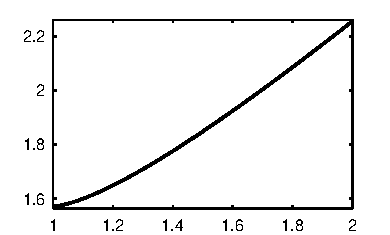
\includegraphics[width=.9\textwidth]{PDF/MaxEnt_ArcsineLaw}}
  \end{minipage}
  %
  \begin{minipage}{.4\columnwidth}
\caption{\SZ{Univalued e}ntropy  functional   $\phi_\u$  derived  from   the  arcsine
  distribution with partial constraints $T_{\pm,1}(x) = x \un_{\X_\pm}(x)$.}
\label{fig:Entropy-arcsin}
  \end{minipage}
\end{figure}

%\Avoir{On ne parle pas des moment, Fisher and so on... \`A faire~?}


% ----------------------------------------------------------- Logistic as MaxEnt

\subsection{The logistic distribution}
\label{subsecapp:Logistic}

In this case, \SZ{one can write the distribution under the form
%
\[
f_X(x)  = \frac{1  -  \tanh^2\left(\frac{2 x}{s}\right)}{s} \qquad  \mbox{and}
\qquad T_1(x) = x^2 \qquad \mbox{on} \qquad \X = \Rset.
\]
}
% VAR = pi^2 s^2 / 3
This  distribution, which  resembles  the normal  distribution  but has  heavier
tails,     has     been     used    in     various     \SZ{applications     (see
  e.g.,~\cite{JohKot95:v2})}. One can then check that over each interval
%
\[
\X_\pm = \Rset_\pm
\]
%
the inverse distribution writes \SZ{
%
\[
f_{X,\pm}^{-1}(y) = \pm \frac{s}{2} \argtanh \sqrt{1 - s y}, \qquad y \in \left( 0 \, ; \,
  \frac{1}{s} \right]
\]
}

We concentrate  now on a second  order constraint, that respect  the symmetry of
the distribution,  and on  first order  constrain(s) that  does not  respect the
symmetry.


% ---------------  Logistic second order

\subsubsection{Second order moment constraint}
\label{subsubsecapp:LogisticSecondOrder}

In this  case, \SZ{injecting the  expression of $T_1\left(  f_X^{-1}(y) \right)$
  into   eq.~\eqref{eq:derivative-phi},   we   immediately   obtain
%
\[
\phi'(y) = \lambda_0 + \frac{\lambda_1 s^2}{4} \left( \argtanh\sqrt{1 - s y} \right)^2
\qquad \mbox{with} \qquad \lambda_1 < 0
\]
%
where      $\lambda_1      <      0$       is      required      to      satisfy
condition~\ref{MonotonyDomains:cond}.   After   a  reparameterization,   we  thus
achieve  the  family  of  entropy  functionals $\phi(y)  =  \phi_\u(s  y)$  with
$\phi_\u(u)  = -\alpha  \left[ u  \left(  \argtanh\sqrt{1-u} \right)^2  \!  -  2
  \sqrt{1-u} \,  \argtanh\sqrt{1-u} -  \log u  \right] \un_{\left( 0  \, ;  \, 1
  \right]}(u) + \beta u + \gamma$ with \ $\alpha > 0$.

Here again, $s$ is an additional parameter for this family of $\phi$-entropies.

The entropic  functional is defined  for $u  \le 1$ due  to the domain  $f_X$ is
invertible. To evaluate the $\phi$-entropy for a given distribution $f$, one can
play on parameter $s$ so as to restrict, if possible, $s f$ to be on $[0 \, ; \,
  1]$. But  one can also extend  the functional to $\Rset_+$  while remaining of
class $C^1$ by vanishing the derivative at $u = 1$: this imposes $\beta = 0$ and
leads to the entropic functional
%
\begin{eqnarray*}
  &&\hspace{-7mm}\phi(y) = \phi_\u(s y) \qquad \mbox{with}
 \\[2.5mm]  
&&\hspace{-7mm}\phi_\u(u)  =  \gamma - \alpha \left[  u  \left( \! \argtanh\!\sqrt{1-u} \right)^{\! 2} \!\!  -  2
  \sqrt{1-u}  \, \argtanh\!\sqrt{1-u} -  \log  u  \right] \un_{\left(  0  \,  ; \,  1
  \right]}(u), \:\: \alpha > 0
\end{eqnarray*}
%
depicted figure~\ref{fig:Entropy-logistic}(a) for $\alpha = 1, \: \gamma = 0$.
}

%\Avoir{On ne parle pas des moment, Fisher and so on... \`A faire~?}


%\Avoir{Interestingly, when  $s \to 0$, the  logistic law tends to  the Gaussian
%distribution. to finish}



% --------------- Logistic first order

\subsubsection{(Partial) first-order moment(s) constraint(s)}
\label{subsubsecapp:LogisticFirstPartial}

Since $f_X$ and $T(x) = x$ do no share the same symmetries, one cannot interpret
the logistic  distribution as a  maximum entropy  constraint by the  first order
moment. However, constraining the partial means over $\X_\pm = \Rset_\pm$ allows
such an interpretation, using then multiform entropies, while the alternative is
to relax  the concavity  property of  the entropy \SZ{(but  again) one  can only
  insure that the  distribution from which it comes from  is a critical point}.
\SZ{To be more precise, one chooses
%
\[
T_{\pm,1}(x) = x \, \un_{\X_\pm}(x) \qquad \mbox{or} \qquad T_1(x) = x
\]
%
We     thus    obtain     from    eq.~\eqref{eq:derivative-phil-partial}     and
eq.~\eqref{eq:derivative-phil}  respectively,   over  each  set   $\X_\pm$,  the
branches
%
\[
\phi'_\pm(y)  =  \lambda_0  +  \frac{\lambda_{\pm,1}  s}{2}  \argtanh\sqrt{1-sy}
\qquad \mbox{\&} \qquad \widetilde{\phi}'_\pm(y) = \lambda_0 \pm \frac{\lambda_1
  s}{2} \argtanh\sqrt{1-sy}
\]
%
where the sign is absorbed on $\lambda_\pm$ for the first case. Dealing with the
partial  moments,  to   satisfy  condition~\ref{MonotonyDomains:cond}  one  must
impose $$\lambda_\pm < 0$$ At the opposite, condition~\ref{MonotonyDomains:cond}
cannot be satisfied for the second case (one would have to impose $\pm \lambda_1
< 0$ on $\X_\pm$).  After a  reparameterization of the $\lambda_i$s, one obtains
the  branches  of  the  entropic   functional  under  the  form  $\phi_\pm(y)  =
\phi_{\pm,\u}(s  y)$  with   $\phi_{\pm,\u}(u)  =  -  \alpha_\pm   \left(  u  \,
\argtanh\sqrt{1-u} \, -  \sqrt{1-u} \right) \un_{\left( 0 \, ;  \, 1 \right]}(u)
\, + \, \beta  \, u \, + \, \gamma_\pm$ where $\alpha_\pm  > 0$ and the branches
for the  non-convex case $\widetilde{\phi}_\pm(y)  = \widetilde{\phi}_{\pm,\u}(s
y)$   with   $   \widetilde{\phi}_{\pm,u}(u)   =  \pm   \alpha   \left(   u   \,
\argtanh\sqrt{1-u} \, -  \sqrt{1-u} \right) \un_{\left( 0 \, ;  \, 1 \right]}(u)
  \, + \, \beta \, u \, + \, \gamma_\pm$.

Once  again,  appears  an  additional  parameter, $s$,  for  these  families  of
entropies.

In both cases,  even if the inverse of  $f_X$ restricts $u$ to be  lower than 1,
one can either play  on parameter $s$ to allow to  compute the $\phi$-entropy of
any distribution  $f$, or  to extend  the entropic  functionals to  $\Rset_+$ by
vanishing the  derivative at  $u =  1$.  This impose  $\beta =  0$ and  thus the
entropic functional,
%
\begin{eqnarray*}
  &&\phi_\pm(y)  =
  \phi_{\pm,\u}(s  y) \qquad \mbox{with}
  \\[2.5mm]
  && \phi_{\pm,u}(u)  =   \gamma_\pm -  \alpha_\pm  \left(   u  \,
  \argtanh\sqrt{1-u} \, -  \sqrt{1-u} \right) \un_{\left( 0 \, ;  \, 1 \right]}(u), \qquad \alpha_\pm  > 0
\end{eqnarray*}
%
and the branches for the non-convex case
%
\begin{eqnarray*}
  && \widetilde{\phi}_\pm(y)  = \widetilde{\phi}_{\pm,\u}(s
  y) \qquad \mbox{with}
  \\[2.5mm]
  &&\widetilde{\phi}_{\pm,u}(u)   =  \gamma_\pm \pm   \alpha   \left(   u   \,
  \argtanh\sqrt{1-u} \, -  \sqrt{1-u} \right) \un_{\left( 0 \, ;  \, 1 \right]}(u)
\end{eqnarray*}


Remarkably, in  the first case, an  univalued entropic functional can  be obtain
imposing both $\alpha_+ = \alpha_-, \,  \gamma_+ = \gamma_-$.  Here also, such a
choice is  equivalent to considering the  constraint $T_1(x) = |x|$,  and thus
allows to respect the symmetries of the distribution, allowing thus to recover a
classical $\phi$-entropy.

\

The        uniform        function        $\phi_\u$        is        represented
figure~\ref{fig:Entropy-logistic}(b) for $\alpha_\pm = 1, \: \gamma_\pm = 0$.

\begin{figure}[htbp]
\centerline{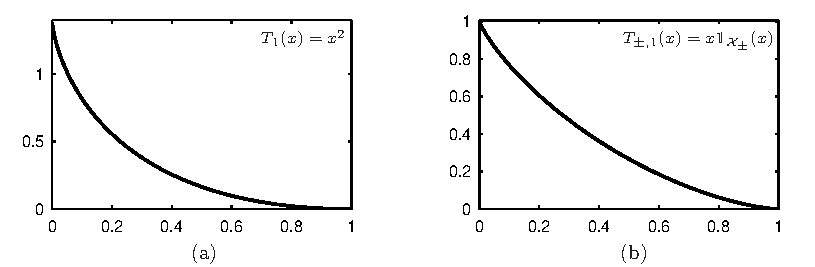
\includegraphics[width=\columnwidth]{PDF/MaxEnt_LogisticLaw}}
\caption{Entropy  functional  $\phi_\u$   derived  from  the  logistic
  distribution:  (a)~with  $T_1(x)  =  x^2$   and  (b)~with  $T_{\pm,1}(x)  =  x
  \un_{\X_\pm}(x)$.}
\label{fig:Entropy-logistic}
\end{figure}
}

  
%\Avoir{On ne parle pas des moment, Fisher and so on... \`A faire~?}


% -------------------------------------------------- Gamma first order as MaxEnt

\subsection{The gamma distribution and (partial) $p$-order moment(s)}
\label{subsecapp:GammaFirstOrder}

As a very special case, consider here the gamma distribution expressed as
%
\SZ{
\[
f_X(x) = \frac{\left( \Gamma(q)  x \right)^{q-1} \exp\left(- \frac{\Gamma(q)}{r}
  \, x \right)}{r^q} \qquad \mbox{on} \qquad \X = \Rset_+.
\]
%
Parameter  $q >  0$ is  known as  shape parameter  of the  law, while  $\sigma =
\frac{r}{\Gamma(q)} > 0$ is a  scaling parameter. This distribution also appears
in various applications, as described for instance in~\cite{JohKot95:v1}.}

Let  us  concentrate  on  the  case  $q >  1$  for  which  the  distribution  is
non-monotonous,  unimodal, where  the  mode is  located at  \SZ{$x  = \frac{r  \,
    (q-1)}{\Gamma(q)}$, and $f_X(\Rset_+)  = \left[ 0 \,  ; \, \frac{(q-1)^{q-1}
      \, e^{1-q}}{r} \right]$ }

Here again it cannot be \SZ{a  maximizer of a $\phi$-entropy constraint subject
  to  a moment  of order  $p >  0$}.  Here,  we can  again \SZ{consider  partial
  moments as constraints,
  %
  \SZ{
\begin{eqnarray*}
&&  T_{k,1}(x) =  x^p  \,  \un_{\X_k}(x), \qquad  k  \in \{  0  ,  -1 \}  \qquad
  \mbox{where} \\[2.5mm] && \X_0 = \left[ 0 \, ; \, \frac{r \, (p-1)}{\Gamma(q)}
    \right)   \qquad   \mbox{and}   \qquad   \X_{-1}   =   \left[   \frac{r   \,
        (q-1)}{\Gamma(q)} \, ; \: +\infty \right),
\end{eqnarray*}
%
}
or interpret $f_X$ as a critical point of an $\phi$-like entropy by constraining} the moment 
%
\[
T_1(x) = x^p \quad \mbox{over} \quad \X = \Rset_+
\]
%
Inverting $y = f_X(x)$ leads to the equation
%
\SZ{
\[
- \frac{\Gamma(q) \, x}{r \, (q-1)}  \exp\left( -  \frac{\Gamma(q) \, x}{r \, (q-1)}  \right) =  -
       \frac{\left( r y \right)^{\frac{1}{q-1}}}{q-1}
\]
}
%
to be solved. As expected, this  equation has two solutions. These solutions can
be  expressed   via  the   multivalued  Lambert-W   function  $\W$   defined  by
$z=\W(z)\exp(\W(z))$,  i.e., $\W$  is  the  inverse function  of  $u \mapsto  u
\exp(u)$\cite[\S~1]{CorGon96}, leading to the inverse functions
%
\SZ{
\[
f_{X,k}^{-1}(y) = - \frac{r \,  (q-1)}{\Gamma(q)} \, \W_k\left( - \frac{\left( r
  y \right)^{\frac{1}{q-1}}}{q-1}  \right) ,  \qquad r  y \in \left[  0 \,  ; \,
  \left( \frac{q-1}{e} \right)^{q-1} \right],
\]
}
%
where  $k$  denotes the  branch  of  the  Lambert-W  function. $k=0$  gives  the
principal branch and here it is related  to the entropy part on $\X_0$, while $k
= -1$ gives the secondary branch, related to $\X_{-1}$ here.

\SZ{Applying~\eqref{eq:derivative-phil-partial}  to  obtain  the branches  of  the
  functionals  of the  multiform entropy,  one}  has thus  to \SZ{integrate  the
  functions}
%
\[
\phi'_k(y) = \lambda_0 + \lambda_{k,1}  \left[ - \frac{r \, (q-1)}{\Gamma(q)} \,
  \W_k\left( - \frac{\left( r y \right)^{\frac{1}{q-1}}}{q-1} \right) \right]^p
\]
%
where, to insure the convexity of the $\phi_k$,
%
\[
(-1)^k \lambda_{k,1} > 0
\]
%
The  same  approach  allows  to   design  $\widetilde{\phi}_k$,  with  a  unique
$\lambda_1$  instead  of the  $\lambda_{k,1}$s  \SZ{and  without restriction  on
  $\lambda_1$}.

Integrating  the previous  expression  is  not an  easy  task.   Relation $u  \,
(1+\W_k(u)) \, \W_k'(u) =  \W_k(u)$~\cite[Eq.~3.2]{CorGon96} suggests that a way
to make the integration is to search for\SZ{
%
\[
\phi_k(y) = \phi_{k,\u}\left( r y \right)
\]
%
where the primitive  of the term with the Lambert  function in} $\phi_{k,\u}(u)$
is searched  \SZ{under the form  $u \, \sum_{l \ge  0} a_l \left[-  \W_k\left( -
    \frac{u^{\frac{1}{q-1}}}{q-1}   \right)   \right]^{l+p}$,  identifying   the
  coefficients $a_l$.}  Such  an approach\SZ{, after a  reparameterization of the
  $\lambda_i$s,} leads to the family of entropic functional \SZ{given by}
%
\begin{eqnarray*}
\phi_{k,\u}(u) & = & \beta \, u \, + \, \gamma_k \, + \, \alpha_k \, u \, \left[
  - \W_k\left( - \frac{u^{\frac{1}{q-1}}}{q-1} \right) \right]^p \, \times
\\[2.5mm]
&&\hspace{-2.5mm}\left[ 1 - \frac{p}{p+q-1} \:
  \hypgeom{1}{1}\left(  1 \,  ; \,  p+q \,  ; \,  (1-q) \W_k  \left( -
  \frac{u^{\frac{1}{q-1}}}{q-1}  \right)   \right)  \right] \: \un_{\left(  0   \,  ;  \,
  \left( \frac{q-1}{e} \right)^{q-1} \right)}(u)
\end{eqnarray*}
%
\SZ{with $$(-1)^k  \alpha_k >  0$$ and where  $\hypgeom{1}{1}$ is  the confluent
  hypergeometric       (or       Kummer's)       function~\cite[\S~13]{AbrSte70}
  or~\cite[\S~9.2]{GraRyz15}}.  One can verify a posteriori that these functions
are the ones we search for.

\SZ{Again, $p, q, r$ are additional parameters for this family of entropies.

  Then, from the domain of definition of the inverse of $f_X$, $u$ is restricted
  to $\left( 0 \, ; \, \left( \frac{q-1}{e} \right)^{q-1} \right)$, which can be
  compensated for by  playing with parameter $r$.  At the  opposite, noting that
  $\W_k\left( -e^{-1} \right) = -1$, to extend the entropic functionals to $C^1$
  functions on  $\Rset_+$, one would  have to impose $\beta  + \alpha_k =  0$ to
  vanish the derivatives at $u = e^{1-a}$. This is impossible because from $(-1)
  \alpha_k >  0$ one  cannot impose  $\alpha_k =  - \beta$.   One can  choose to
  impose $$\beta  = -  \alpha_{-1}$$ to vanish  the derivative  for $\phi_{-1}$,
  that is given for the semi-infinite  domain $\X_{-1}$. Moreover, even a convex
  extension relaxing  the $C^1$ condition is  impossible since we would  have to
  impose $\beta +  \alpha_k \le \beta$ to insure the  increase of the $\phi_k$s.
  We can however choose  the $\gamma_k$ such that the $\phi_k$  coincide at $u =
  0$ for instance  (e.g., to vanish them  at $0$ to insure the  existence of the
  $\phi$-entropy), that gives
%
\[
\gamma_0  = \gamma_{-1} \, -  \, \frac{p \, \Gamma(p+q-1)}{(q-1)^p} \,
\alpha_{-1}
\]
%
using successively~\cite[Eq.~3.1]{CorGon96}  and~\cite[Eq.~13.1.2]{AbrSte70} for
$\W_0$,  and  successively~\cite[Eq.~13.1.4]{AbrSte70}   ($\W_{-1}$  tending  to
$-\infty$ in  $0^{-}$), $\W_{-1}(u) \exp(\W_{-1}(u)) =  u$, and~\cite[Eq.~4.6 \&
  lines that  follow]{CorGon96} for  $\W_{-1}$.
}

The  same algebra  leads to  the same  expression for  the $\widetilde{\phi}_k$,
except that the $\lambda_{k,1}$s are replaced by a unique $\lambda_1$.

\


\Avoir{Interestingly, when  $a \to 1$,  the gamma  law tends to  the exponential
  distribution  and, at  the  same time,  $\X_0 \to  \emptyset,  \: \X_{-1}  \to
  \Rset_+$. to finish}

\

The  multivalued  function  $\phi_\u$  in the  concave  context  is  represented
figure~\ref{fig:Entropy-gamma} for  $p = 2,  q =  2$ and $q  = 5$, and  with the
choice \SZ{$\alpha_0 = 1,  \: \alpha_{-1} = -0.05, \: \beta  = - \alpha_{-1}, \:
  \gamma_0   =  0,   \:   \gamma_{-1}  =   \frac{p  \Gamma(p+q-1)}{(q-1)^p}   \,
  \alpha_{-1}$}.

\begin{figure}[htbp]
\centerline{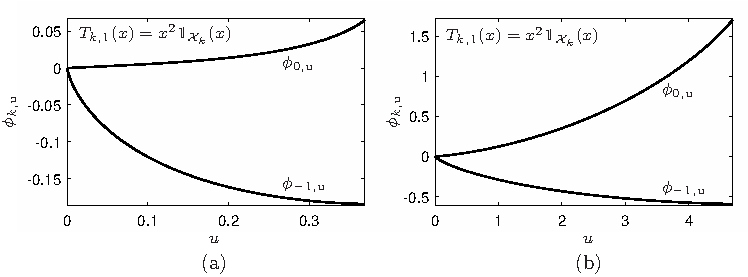
\includegraphics[width=.78\textwidth]{PDF/MaxEnt_GammaLaw}}
\caption{Multiform  entropy   functional  $\phi_\u$   derived  from   the  gamma
  distribution   with  the   partial  moment   constraints  $T_{k,1}(x)   =  x^2
  \un_{\X_k}(x)$, $k\in\{0,-1\}$.  (a): $q = 2$; (b): $q = 5$.}
\label{fig:Entropy-gamma} 
\end{figure}

\

%\Avoir{On ne parle pas des moment, Fisher and so on... \`A faire~?}

\Avoir{
  \begin{itemize}
  \item Ponctuer titres et titre des sections?
    %
  \item $T_i$s ou $T_i$'s~? De m\^eme pour les $\lambda_i$s.
    %
  \item Integrable ou summable?
    %
  \item Limite  de la Gamma  vers l'exponentielle et  moment d'ordre 1:  on doit
    trouver Shannon (en param\'etrisant correctement).
  \end{itemize}
  }


% ------------------------------- Bibliography ------------------------------- %
% ---------------------------------------------------------------------------- %

\end{paracol} % To 'close' the left column open by the frontpage...
\reftitle{References}
\externalbibliography{yes}
\bibliography{New_entropies}



% --------------------------------- Biography -------------------------------- %
% ---------------------------------------------------------------------------- %

%% If authors have biography, please use the format below
%\Avoir{
%  \section*{Short Biography of Authors}
%\bio
%{\raisebox{-0.35cm}{
\includegraphics[width=3.5cm,height=5.3cm,clip,keepaspectratio]{PhotoSteeve}}}
%{\textbf{Steeve Zozor} Biography of first author}
%%
%\bio
%{\raisebox{-0.35cm}{
\includegraphics[width=3.5cm,height=5.3cm,clip,keepaspectratio]{PhotoSteeve}}}
%  {\textbf{Jean-Fran\c{c}ois Bercher} Biography of second author}
%  }

\end{document}
